\documentclass[12pt]{article}

\usepackage{amssymb,amsmath,amsfonts,eurosym,geometry,ulem,graphicx,caption,color,setspace,sectsty,comment,footmisc,caption,pdflscape,subfigure,array,hyperref,authblk}
\usepackage{makecell}
\usepackage{apacite}
\usepackage [english]{babel}
\usepackage [autostyle, english = american]{csquotes}
\MakeOuterQuote{"}

\graphicspath{ {../charts/} }

\renewcommand\theadalign{cc}
\renewcommand\theadfont{\bfseries}
\renewcommand\theadgape{\Gape[4pt]}
\renewcommand\cellgape{\Gape[4pt]}

\normalem

\onehalfspacing
\newtheorem{theorem}{Theorem}
\newtheorem{corollary}[theorem]{Corollary}
\newtheorem{proposition}{Proposition}
\newenvironment{proof}[1][Proof]{\noindent\textbf{#1.} }{\ \rule{0.5em}{0.5em}}

\newtheorem{hyp}{Hypothesis}
\newtheorem{subhyp}{Hypothesis}[hyp]
\renewcommand{\thesubhyp}{\thehyp\alph{subhyp}}

\newcommand{\red}[1]{{\color{red} #1}}
\newcommand{\blue}[1]{{\color{blue} #1}}

\newcolumntype{L}[1]{>{\raggedright\let\newline\\arraybackslash\hspace{0pt}}m{#1}}
\newcolumntype{C}[1]{>{\centering\let\newline\\arraybackslash\hspace{0pt}}m{#1}}
\newcolumntype{R}[1]{>{\raggedleft\let\newline\\arraybackslash\hspace{0pt}}m{#1}}

\geometry{left=1.0in,right=1.0in,top=1.0in,bottom=1.0in}

\begin{document}

\begin{titlepage}
\title{Stabilizing poverty amid Covid-19 with
\protect \\universal basic income}
\author{Max Ghenis\thanks{Affiliations: Massachusetts Institute of Technology and UBI Center (max@ubicenter.org).
\protect \\
\protect \\Thanks to Alexandria Symonds for helpful comments and suggestions.
}}

\date{March 19, 2020}
\maketitle
\begin{abstract}
\noindent Policymakers are increasingly considering universal basic income (UBI)
as a response to the economic collapse caused by the
Covid-19 coronavirus outbreak. 
Without fiscal policies aimed at low-income Americans,
falling incomes are likely to increase the poverty rate.
Using the 2018 Current Population Survey,
I calculate the minimum UBI amount necessary to avoid a rise in the
Supplemental Poverty Measure resulting from income drops.
I find that a modest UBI could stabilize the poverty rate;
for example, if incomes fall by 10 percent, 
a universal transfer of about \$850, totaling under \$300 billion,
would suffice.
Giving the UBI to everyone is a cheaper poverty stabilization approach than 
excluding children or noncitizens, which requires larger amounts per recipient;
it is about a quarter cheaper in aggregate terms than
limiting transfers to adult citizens.
\vspace{1in}\\
\vspace{0in}\\

\bigskip
\end{abstract}
\setcounter{page}{0}
\thispagestyle{empty}
\end{titlepage}
\pagebreak \newpage




\doublespacing


\section{Introduction} \label{sec:introduction}

The Covid-19 coronavirus has wreaked havoc on the global economy.
Between February 19 and March 19, 2020,
the S\&P 500 index fell from a peak of 3,386 to 2,409,
a 29 percent drop that effectively erased about three years of 
gains~\cite{sp500}.
In the week of March 16, unemployment data from more than a dozen US states
showed that claims were growing by a factor of 10 or more~\cite{robbins_2020}.
Of economic experts in the University of Chicago Institute on Global Markets
panel \citeyear{igm}, 51 percent agreed and 5 percent disagreed on March 12
that "Even if the mortality of COVID-19 proves to be limited
(similar to the number of flu deaths in a regular season),
it is likely to cause a major recession."

In addition to other measures like payroll tax cuts, paid sick leave, and assistance for airlines and small businesses, United States policymakers are now calling for UBIs---either as one-time or recurring payments, and sometimes including means tests---as policy responses to the crisis.

On March 12, Representative Tulsi \citeA{gabbard} introduced a resolution calling for a \$1,000-per-month payment to each adult citizen for as long as Covid-19 is considered a public health emergency. The same day, Democratic Representatives Ro Khanna and Tim Ryan \citeyear{khanna_ryan} proposed means-tested cash transfers of up to \$6,000 per person, modeled after the Earned Income Tax Credit, and Democratic Representative Alexandria \citeA{aoc} included a UBI in a catalog of recommendations for “dramatic action.”  On March 16, Republican Senator Mitt \citeA{romney} proposed a one-time payment of \$1,000 per adult, and Republican Senator Tom \citeA{cotton_2020} echoed this call for cash payments. On March 17, several more legislators announced proposals: Democratic Senators Michael Bennet, Cory Booker, Sherrod Brown, Angus King, Chris Murphy, and Brian Schatz \citeyear{bennet} proposed a series of means-tested per-person payments depending on the duration of the crisis; Democratic representative Ilhan \citeA{omar_2020} said that she was introducing a bill to give \$1,000 to every American adult and \$500 for every child; Republican Senator Josh \citeA{hawley} proposed monthly payments for families with children, varying with 2018 income and family size; Democratic Representative Joe Kennedy III \citeyear{iii_2020} proposed a one-time payment of \$2,000 per adult and \$1,000 per child, plus an additional \$2,000 for adults with annual income below \$100,000; and Senator Bernie \citeA{sanders_covid} proposed "direct, emergency \$2,000 cash payments to every person in America every month for the duration of the crisis." On March 18, Democratic Representative Maxine \citeA{waters}, as chair of the House Financial Services Committee, placed monthly payments of \$2,000 per adult and \$1,000 per child at the top of her list of 28 proposals to help the economy during the Covid-19 crisis.

Treasury Secretary Steven Mnuchin released a statement on March 17 acknowledging that the White House is "looking at sending checks to Americans immediately"~\cite{matthews_2020}. The following day, the Treasury Department released a proposal for \$500 billion in direct checks, sent on April 6 and May 18, varying by household size and income~\cite{nyt_500b}.

These proposals followed calls for UBIs and means-tested cash transfers from prominent economists, advocacy groups, and others. Greg \citeA{mankiw} and Jason \citeA{furman_2020}, who chaired the Council of Economic Advisers under President George W. Bush and President Barack Obama, respectively, have proposed immediate cash payments. Andrew Yang, who centered his 2020 presidential campaign around a UBI funded by a value-added tax, has called for a monthly UBI of \$1,000 per adult and \$500 per child for three months~\cite{kroll_2020}.
Former Democratic congressman and 2020 presidential candidate John \citeA{delaney} also proposed sending each American \$1,000 per month for two months. On March 13, the  \citeA{esp}, which advised on the Bennet bill, proposed means-tested (based on 2019 income) payments of up to \$2,000 per person, followed by \$1,500 in three months and then \$1,000 quarterly until employment recovers. House candidate Suraj \citeA{patel_2020} called for monthly checks of \$1,000 per adult and \$500 per child "until the pandemic is contained and the Sahm Rule is no longer triggered."

In this paper, I simulate a range of income losses---up to 20 percent---resulting from Covid-19 or other economic crises. Under different targeting criteria---whether noncitizens are included, and how much children get relative to adults---I calculate the UBI amount necessary to prevent a rise in poverty, as measured by the 2018 Supplemental Poverty Measure.

I find that even modest UBIs can stabilize the poverty rate, and that including noncitizens and children is a more cost-effective method than excluding them.

This paper begins with a discussion of the data and methodology, then describes the UBI optimization procedure and results given 10 percent income losses and goes on to show the results for a range of income losses. I conclude with a discussion of alternative policies and cash transfer structures, and in \autoref{sec:appendixa} I show results from stabilizing the poverty gap rather than the poverty rate.

\section{Data} \label{sec:data}

I use the 2019 US Current Population Survey (CPS) March Supplement, which reports an expanded set of economic characteristics for households throughout the calendar year 2018. Among these characteristics are thresholds and resource totals for calculating the Supplemental Poverty Measure (SPM)~\cite{spm}. While the Official Poverty Measure (OPM) resource measure is limited to cash income, the SPM includes taxes, transfers, and other expenditures like healthcare and childcare.\footnote{The CPS overestimates SPM poverty due to respondents underreporting receipt of assistance programs. See \citeA{ctam}.} The SPM threshold also accounts for local housing costs, unlike the OPM threshold. The SPM is calculated for each "SPM unit," which is similar to a household and estimates groups of people who share resources (I use "resources" interchangeably with "income" in the rest of the paper).

I report the SPM poverty rate, defined as the population share living in SPM units with resources below their respective poverty thresholds. I also consider the "poverty gap," which measures the total difference between resources and poverty thresholds across all SPM units in poverty. Unlike the poverty rate, the poverty gap measures the benefits of programs for people significantly below the poverty line~\cite{bruenig}. Results on the poverty gap are reported in \autoref{sec:appendixa}.


\section{Methodology} \label{sec:methodology}

I simulate reductions in households' resource levels likely to arise from the economic downturn, and annual UBI amounts---which could be lump-sum or spread across multiple payments---required to offset any resulting rises in the SPM poverty level. A poverty-stabilizing UBI amount is identified for each of 120 scenarios, defined as the Cartesian product of (a) 20 income reductions (between 1 and 20 percent, in 1-percent increments), (b) whether non-citizens are included, and (c) the amount children receive relative to adults (zero, half, and full).

For example, given a 10 percent reduction in SPM resources and a UBI for every person (including citizens and a full share for children), I calculate the poverty rate for many UBI amounts until one is found that leaves the poverty rate within a small tolerance of its current value. For each scenario like this one, I apply a binary search algorithm~\cite{binary_search} to identify the poverty-stabilizing UBI amount, with tolerances of 0.01 percent for the poverty rate and \$100,000 for the poverty gap.

I've published my code on GitHub as a Python Jupyter notebook~\cite{notebook}.


\section{Baseline descriptive statistics} \label{sec:baseline_descriptive_statistics}

The 2018 SPM rate is 12.7 percent; that is, 12.7 percent of US residents are in a SPM unit whose resources fall below its SPM poverty threshold.

Children and non-citizens are more likely to be in poverty: 13.6 percent of children are in poverty, compared to 12.5 percent of adults, and 23.7 percent of non-citizens are in poverty, compared to 11.9 percent of citizens.\footnote{These figures are calculated from the public microdata, and may differ slightly from the official 2018 SPM report~\cite{spm}, which uses more original survey data.}

If annual disposable incomes fell by 10 percent, the poverty rate would rise 25 percent; an additional 10.5 million people would be below the SPM poverty line.

\begin{center}
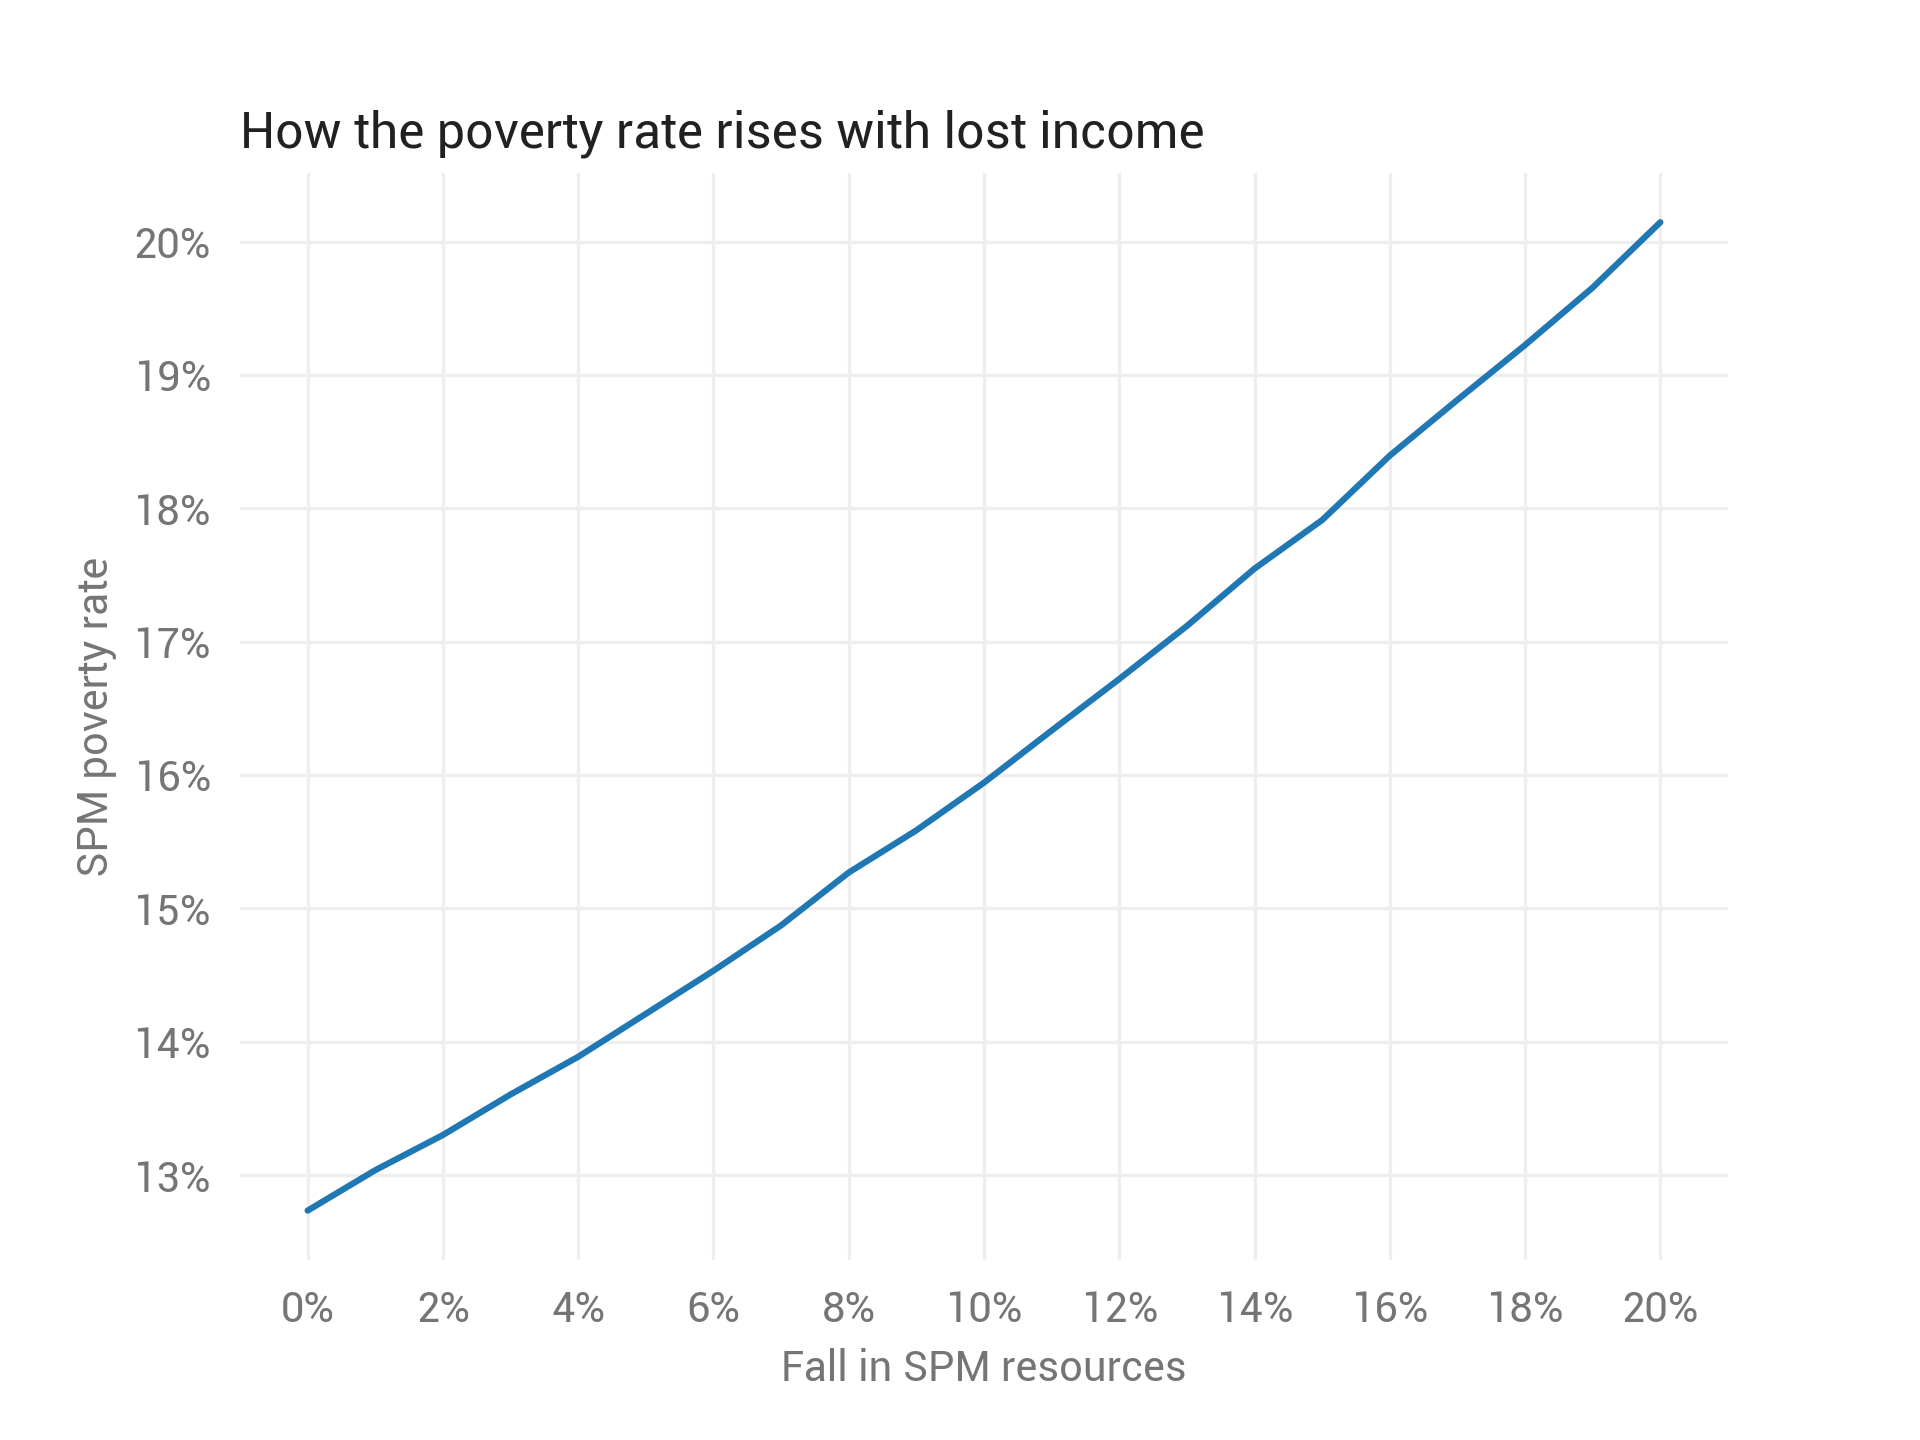
\includegraphics[width=15cm]{pov_rate_income.png}
\captionof{figure}{}
\label{fig:pov_rate_income}
\end{center}


\section{Results} \label{sec:results}

As an illustrative example, I begin by considering an across-the-board 10 percent fall in income (SPM resources), comparing UBI amounts needed to stabilize poverty based on the criteria for receipt. From there, I generalize to each potential income drop between zero and 20 percent, where results are qualitatively similar.

Why start with a 10 percent income drop? This is roughly the economic impact of the Great Recession, on an accelerated time scale. While real median personal and household incomes fell by only 4 to 5 percent from 2007 to 2009, by 2012 they had fallen about 8.5 percent below 2007 levels~\cite{fred_income}. Compared to the S\&P500's 29 percent drop over the month ending March 19, 2020, the index dropped by 53 percent from its October 2007 peak to its March 2009 trough.

As this analysis considers the poverty rate, incomes near the poverty line are most relevant. In the first years of the Great Recession, income inequality fell, especially after taxes and transfers~\cite{cbo}, so incomes fell less near the poverty line than they did near the median. The poverty rate rose by 1.2 percentage points from 2007 to 2012 after considering taxes and transfers.\footnote{Based on anchored SPM estimates calculated by \citeA{cpsp}} However, the pandemic's disproportionate effects on low-wage service industry workers could make its distributional impact more regressive.

\subsection{10 percent fall in income} \label{sec:10pctfall}

When disposable incomes fall by 10 percent, the poverty rate rises from 12.7 percent to 15.9 percent. If a cash transfer is administered to everyone, reducing that rate back to 12.7 percent would require \$828 per person.

\begin{center}
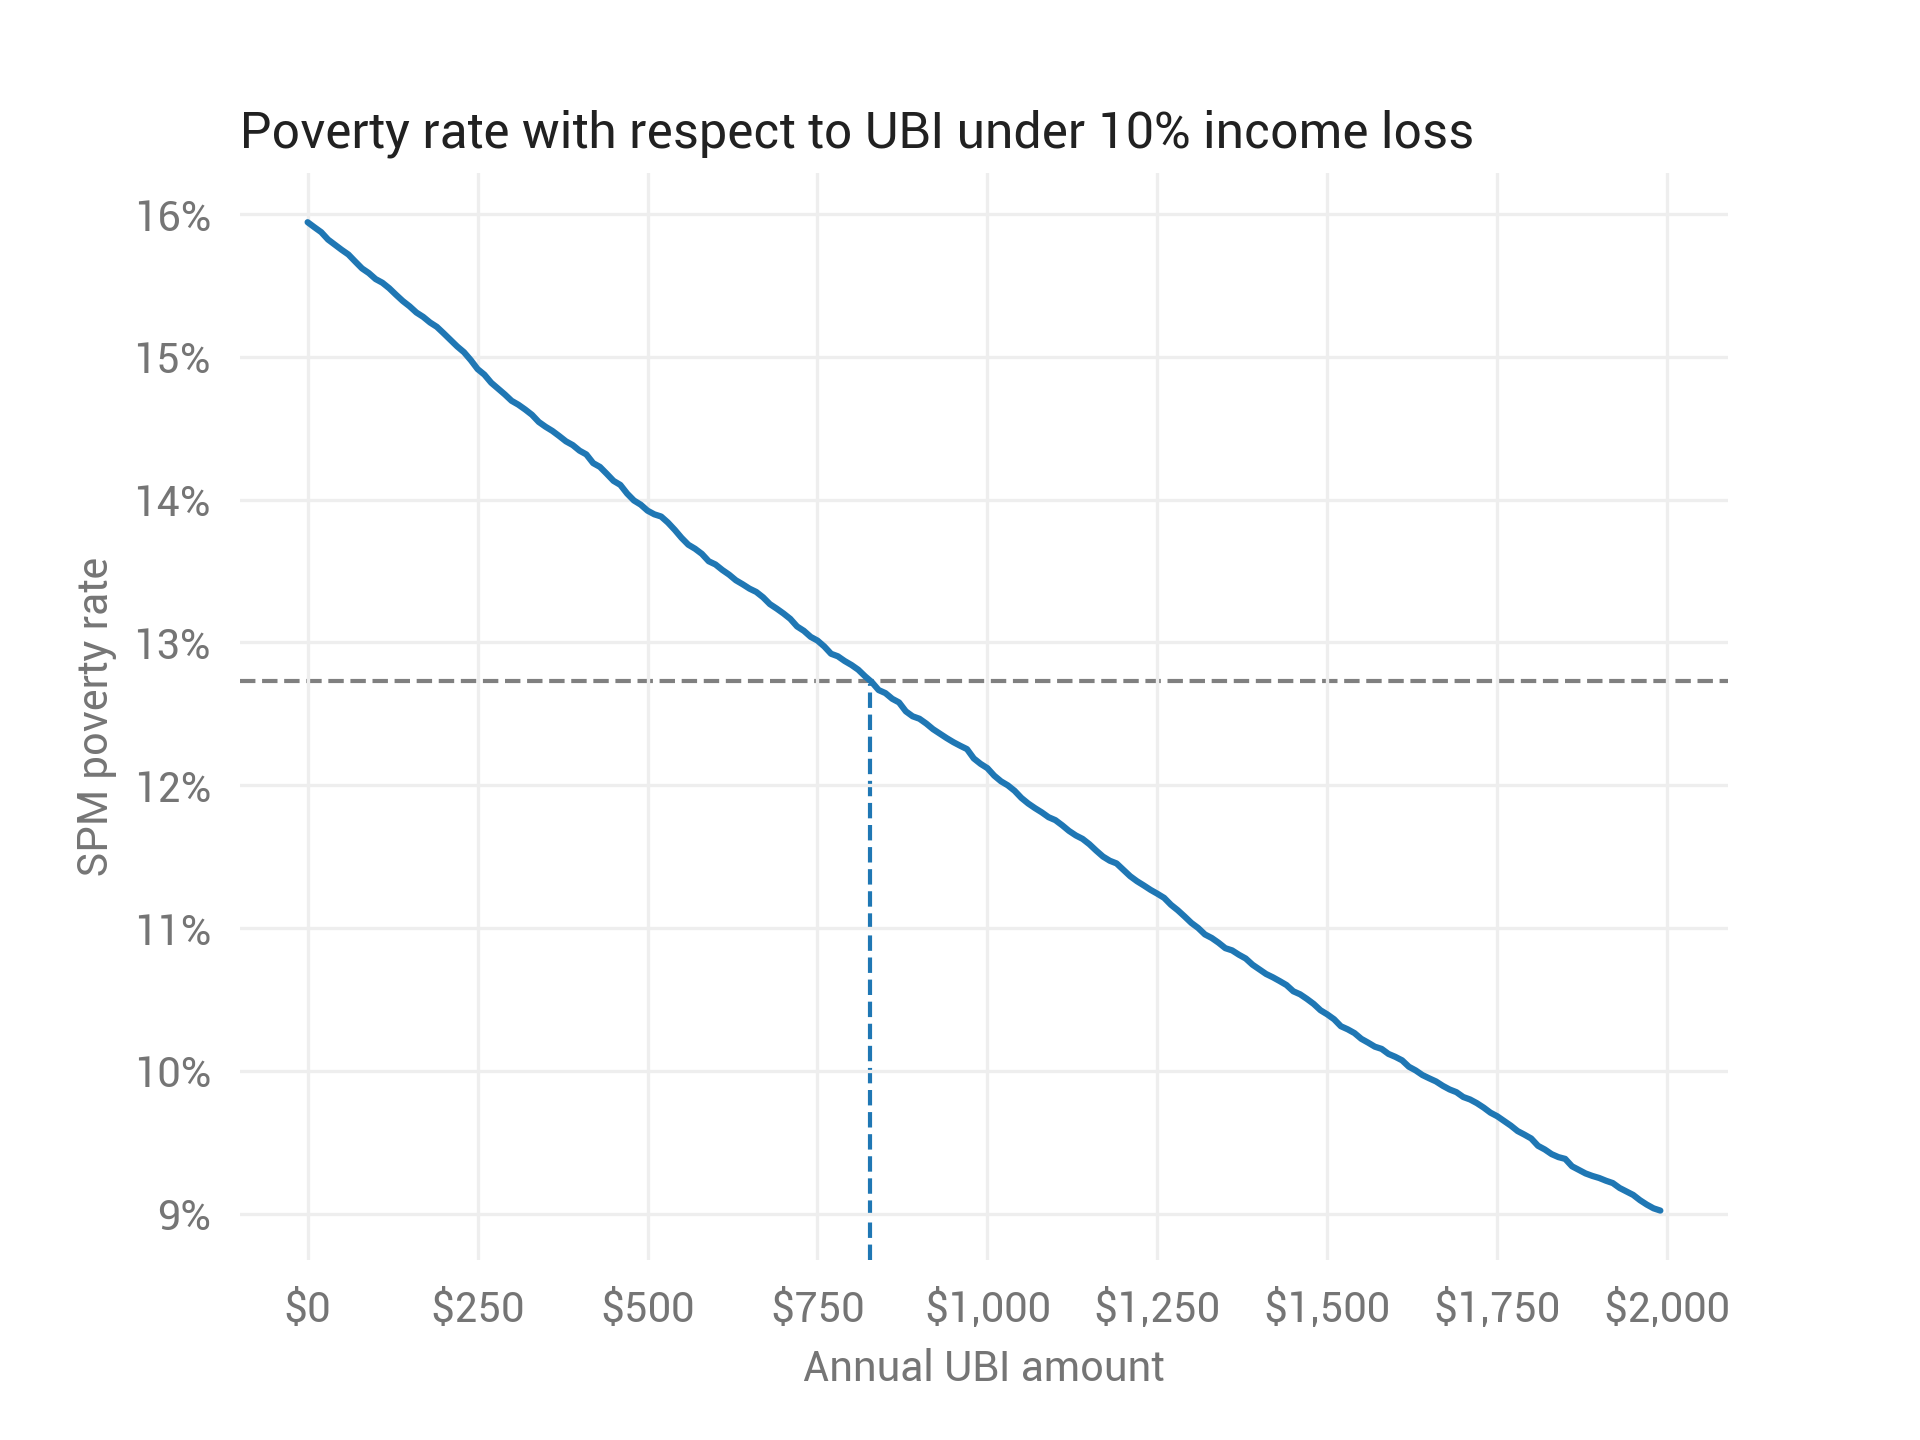
\includegraphics[width=15cm]{pov_rate_by_ubi_10pct_all.png}
\captionof{figure}{}
\label{fig:pov_rate_by_ubi_10pct_all}
\end{center}

If only given to adult citizens, fewer households get the UBI (non-citizens don't), and some households get smaller amounts (those with children). That leaves households who would have been lifted out of poverty remaining below the line. Giving each adult citizen \$828 reduces poverty only to 14.1 percent; to bring it back to 12.7 percent requires \$1,515 per adult citizen.

\begin{center}
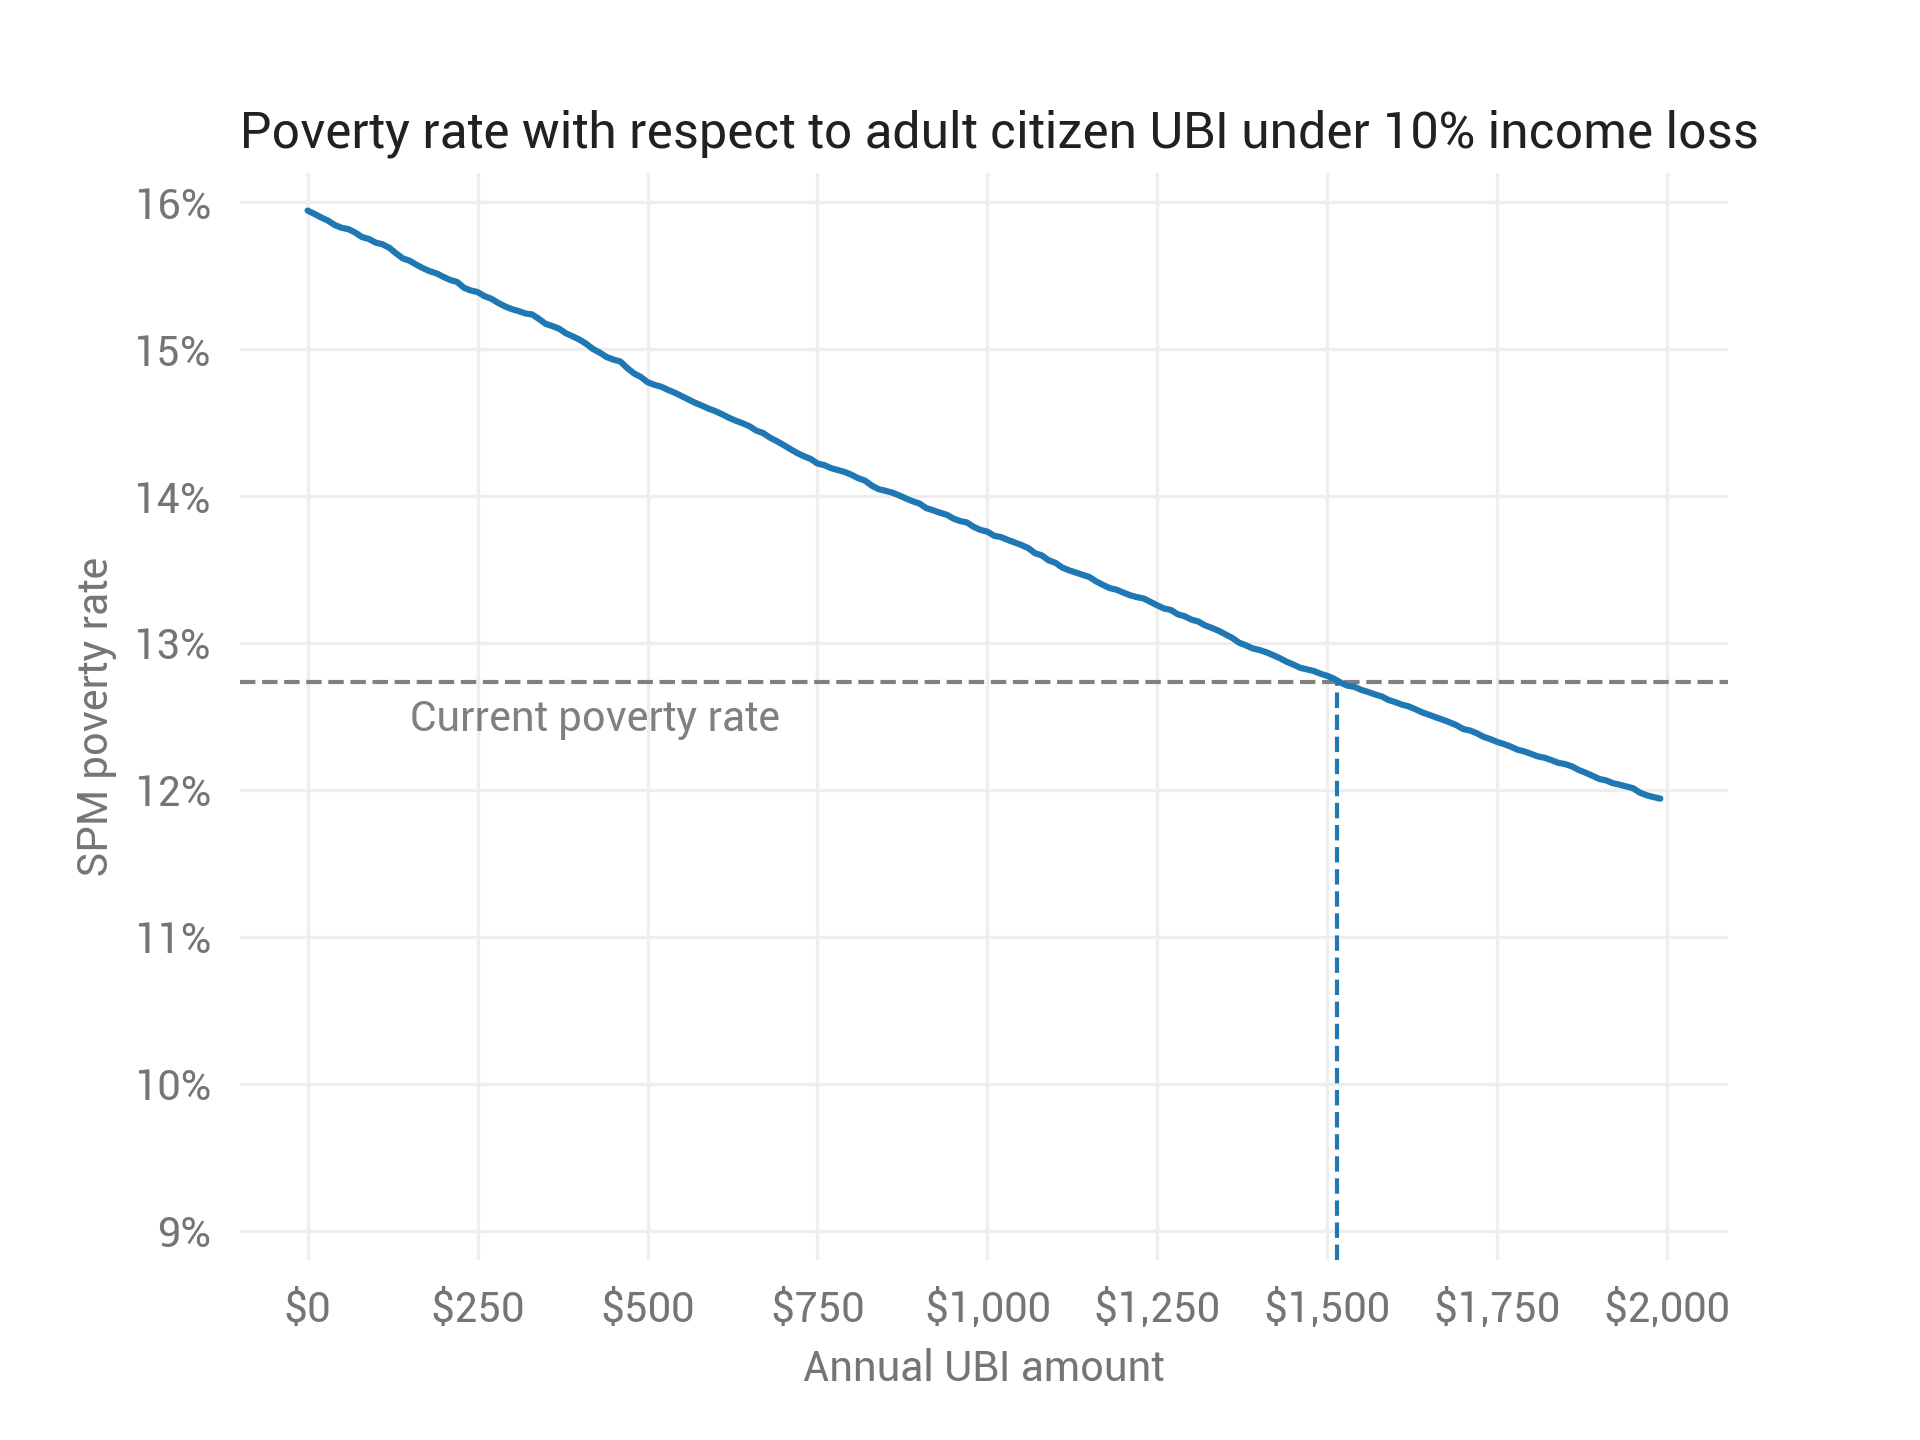
\includegraphics[width=15cm]{pov_rate_by_ubi_10pct_adult_citizens.png}
\captionof{figure}{}
\label{fig:pov_rate_by_ubi_10pct_adult_citizens}
\end{center}

Similarly, stabilizing poverty requires higher payments when children are excluded, or when they only get half the amount as adults.

\begin{center}
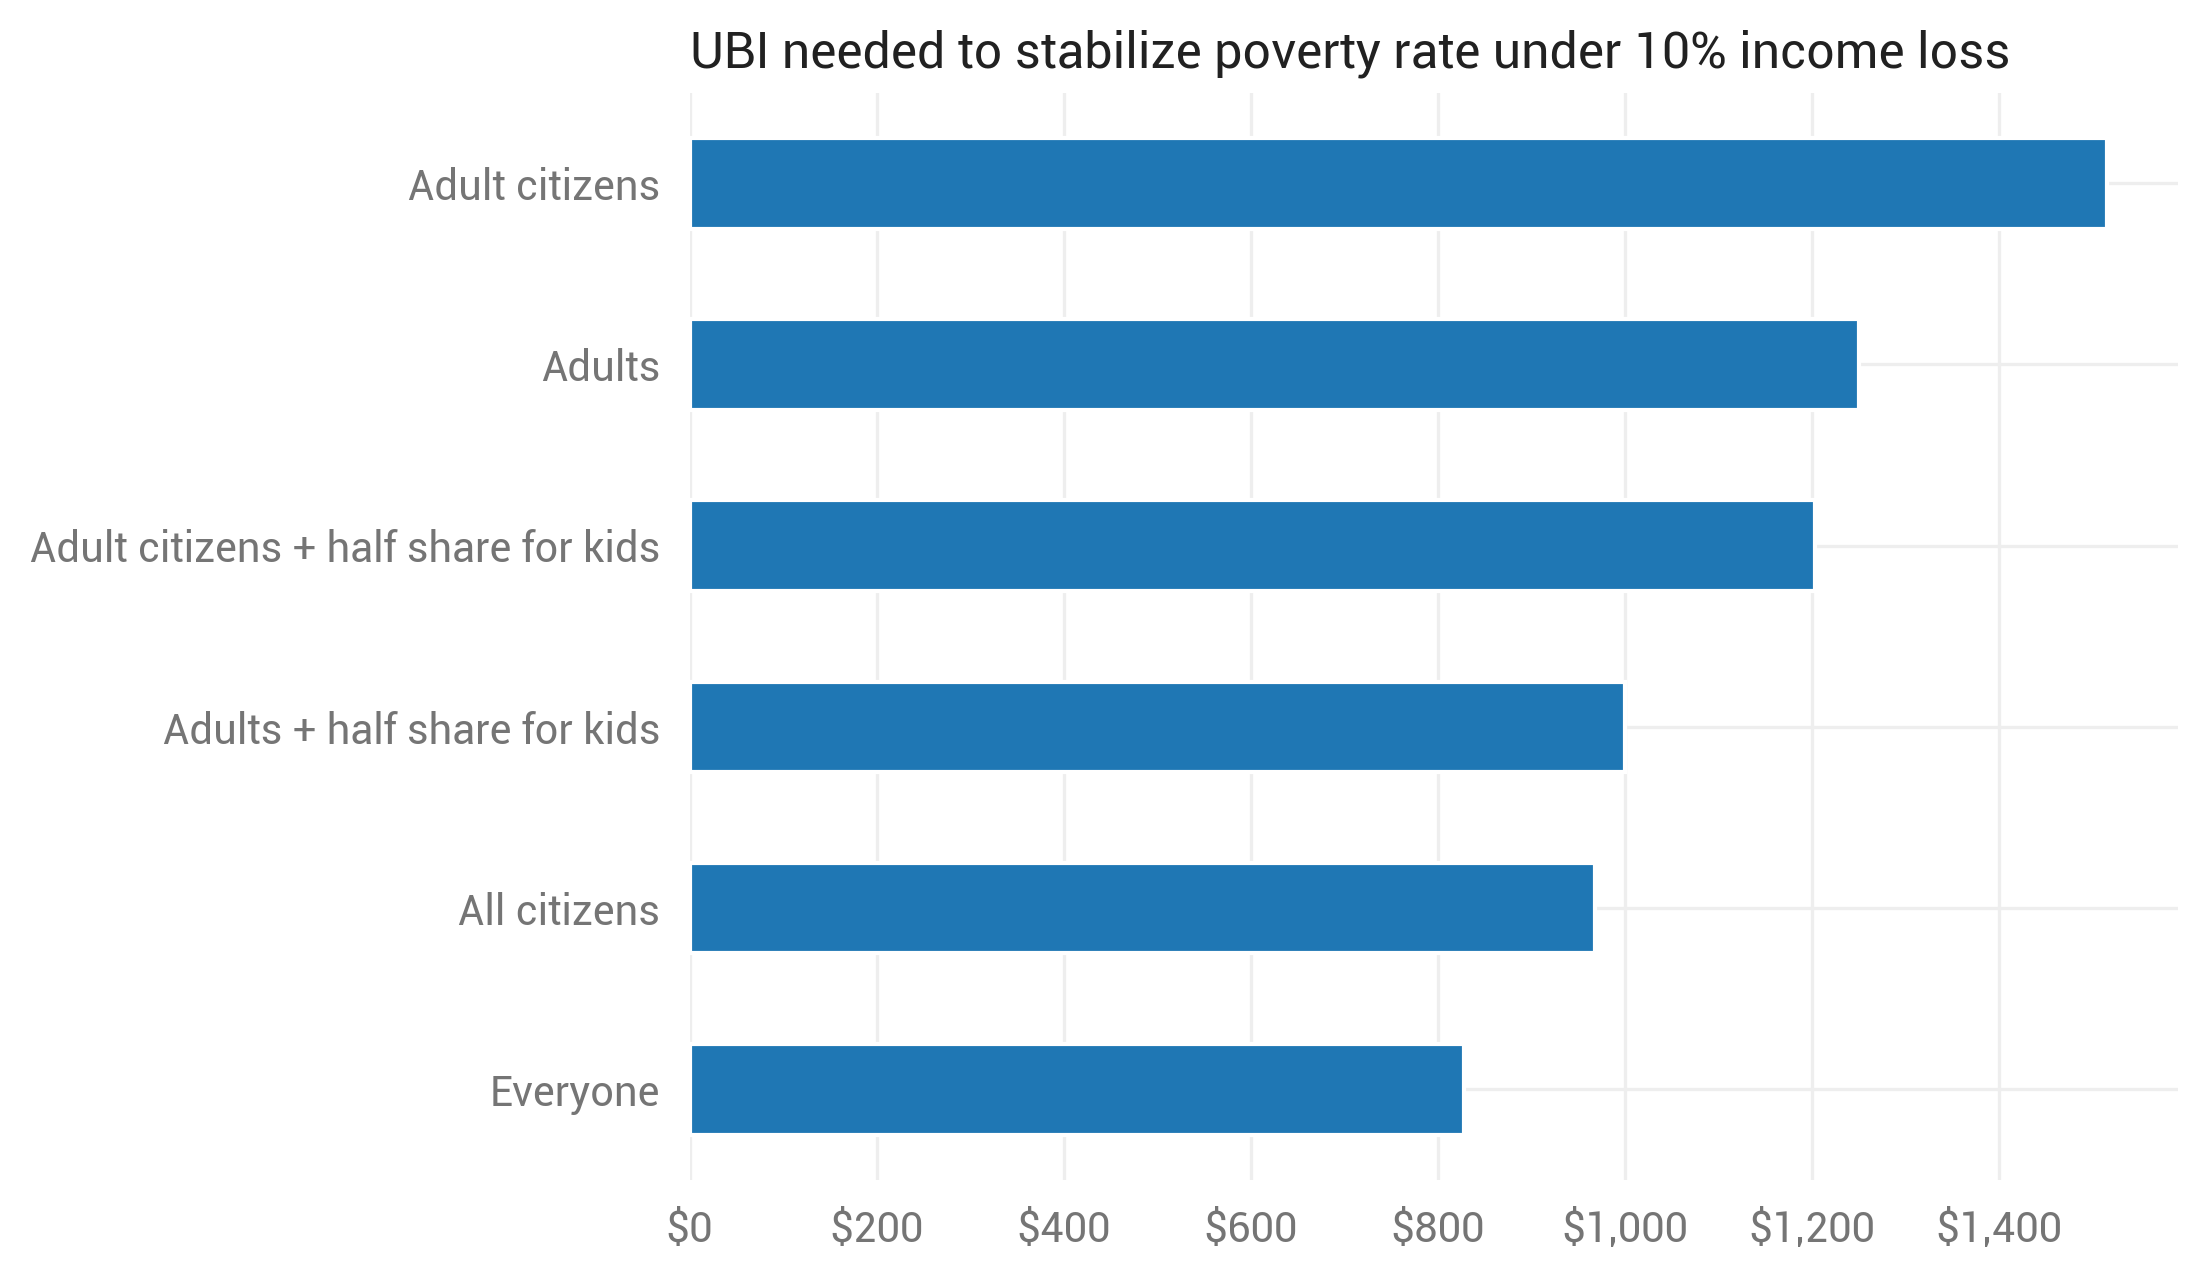
\includegraphics[width=15cm]{ubi_pov_rate_10pct.png}
\captionof{figure}{}
\label{fig:ubi_pov_rate_10pct}
\end{center}

Stabilizing poverty under a smaller UBI base requires giving larger payments to fewer people. Is it worth it?

In this case, it is not. An inclusive program is a considerably cheaper option to stabilize the poverty rate than one that targets particular segments of the population. The \$828 payment to everyone costs \$268 billion. That’s 23 percent less than the \$1,515 to adult citizens, which costs \$347 billion.

\begin{center}
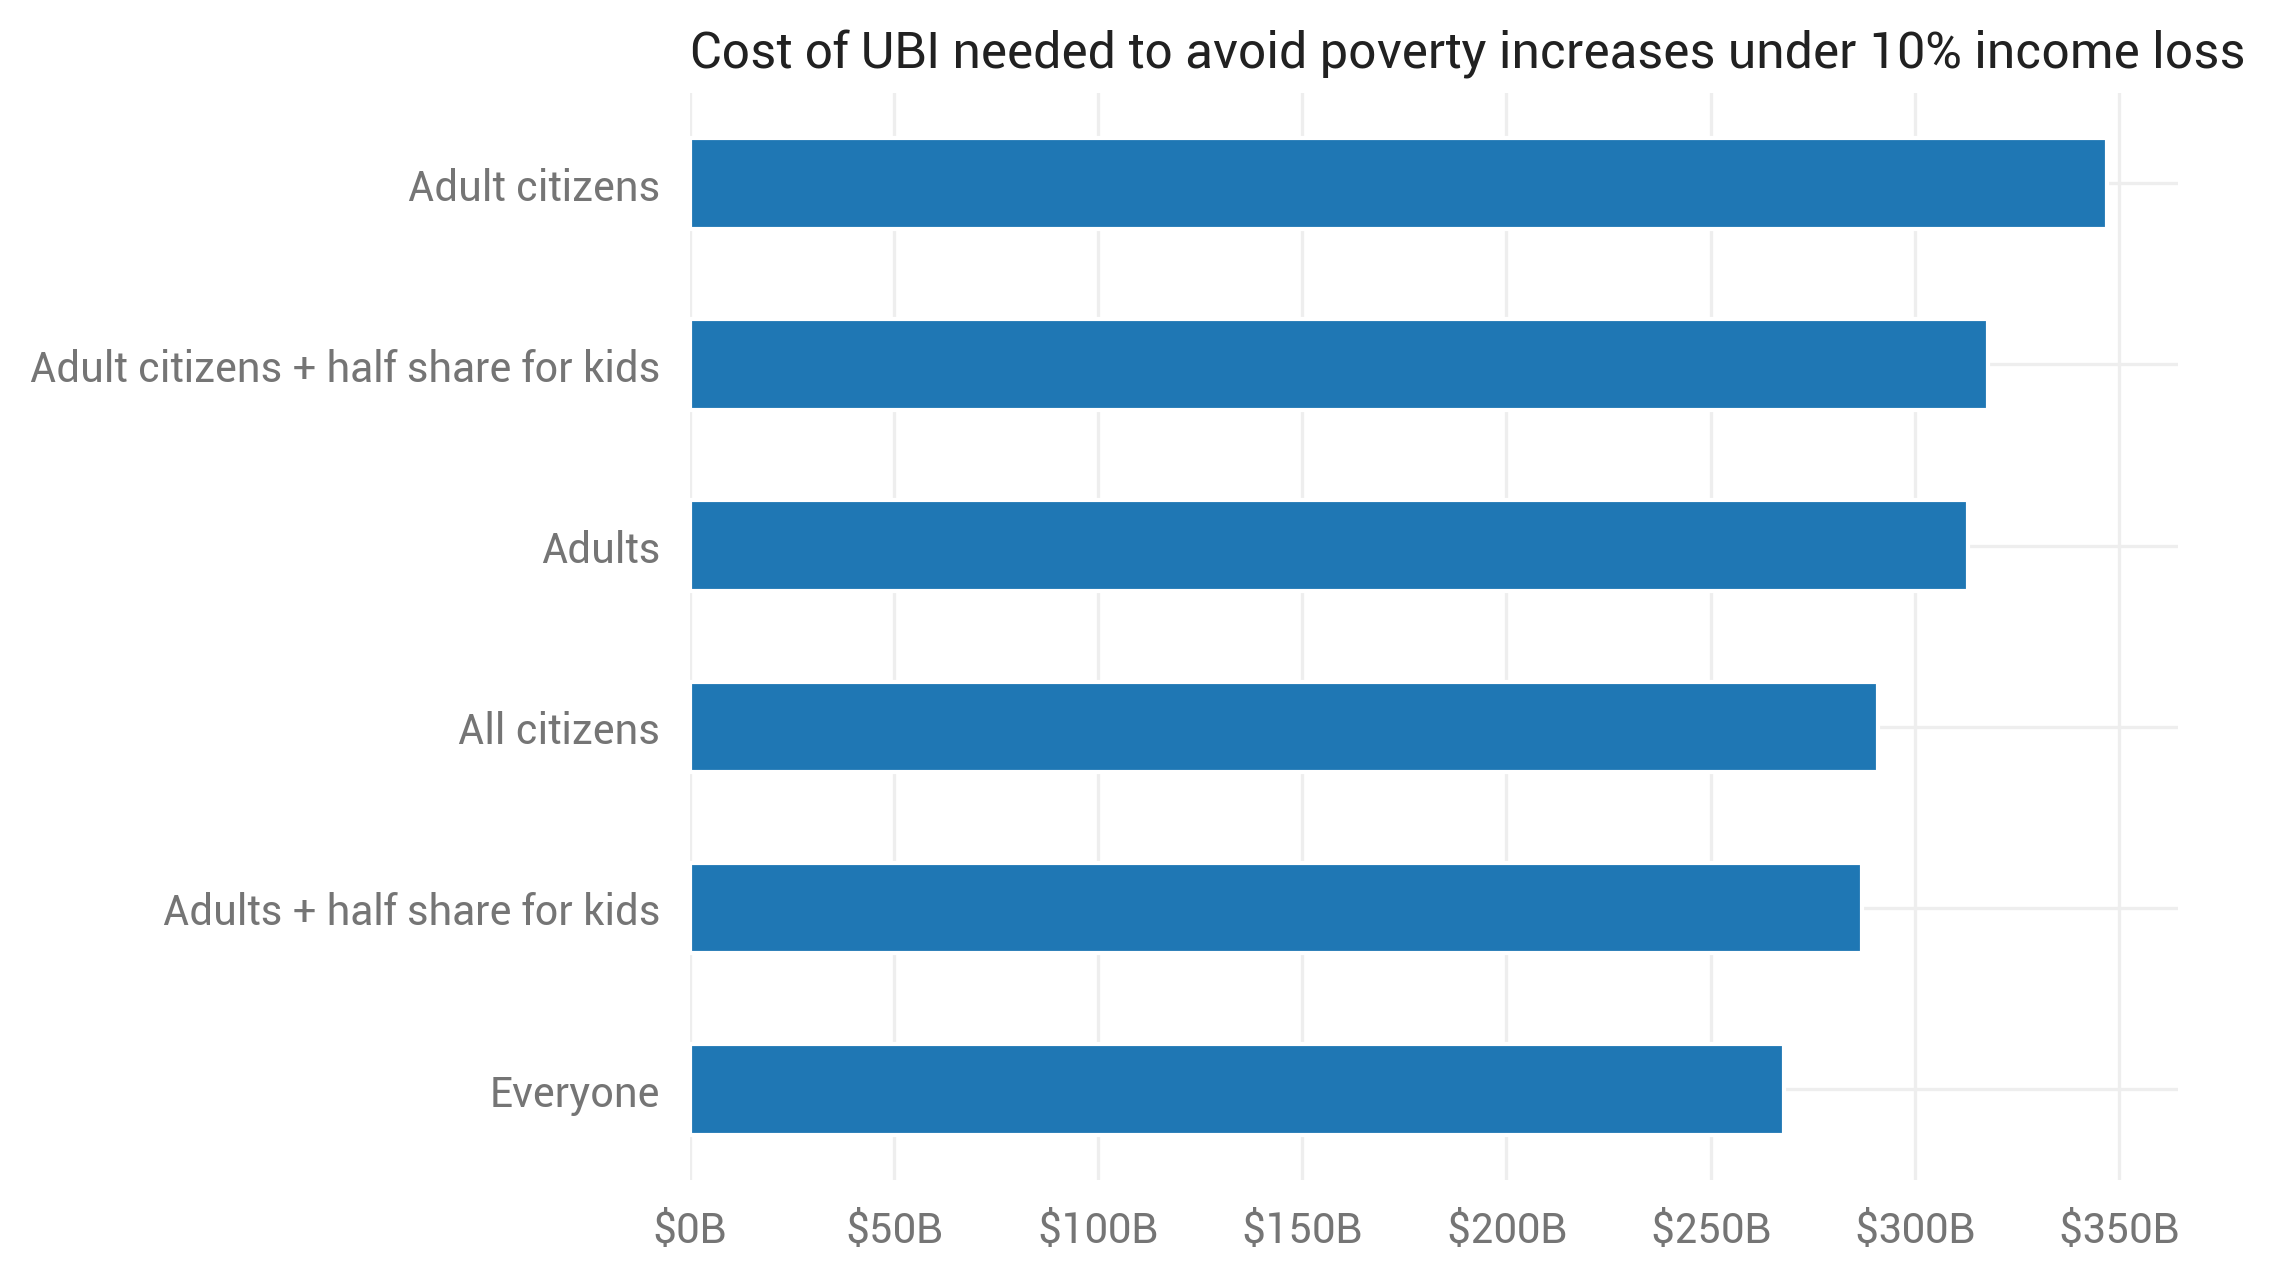
\includegraphics[width=15cm]{ubi_cost_pov_rate_10pct.png}
\captionof{figure}{}
\label{fig:ubi_cost_pov_rate_10pct}
\end{center}

\subsection{Range of income losses} \label{sec:range_losses}

In the case of a 10 percent income loss, providing a UBI to everyone requires a payment of about 45 percent less than providing it only to adult citizens. That ratio roughly holds throughout the spectrum of potential income losses.

\begin{center}
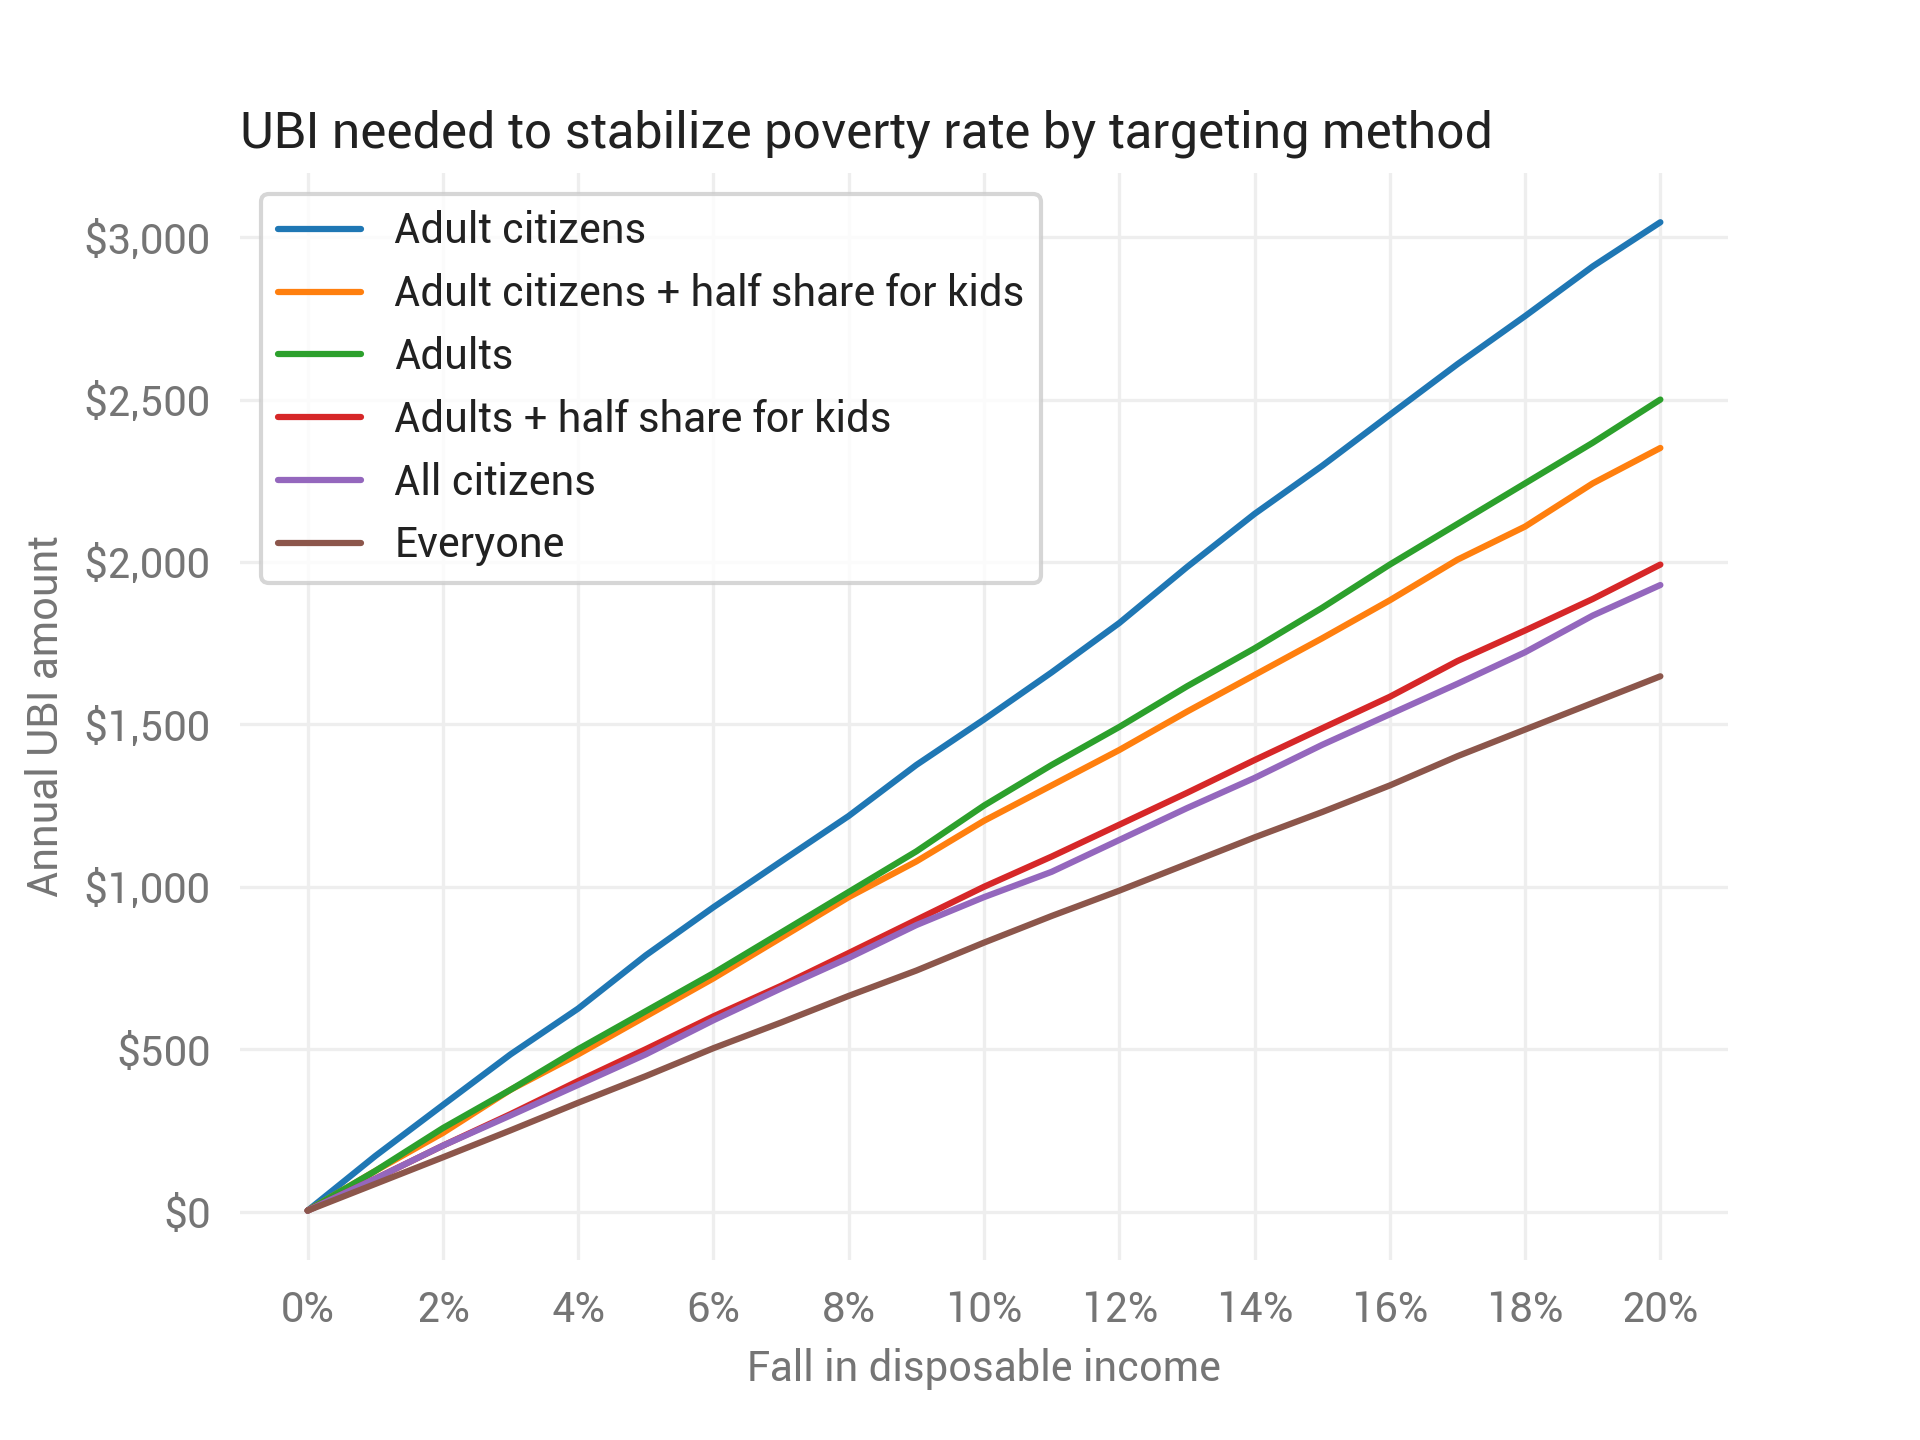
\includegraphics[width=15cm]{ubi_pov_rate.png}
\captionof{figure}{}
\label{fig:ubi_pov_rate}
\end{center}

Giving to everyone is the cheapest modeled approach to stabilizing poverty, regardless of the fall in income, and in general broader transfers make poverty stabilization cheaper.

\begin{center}
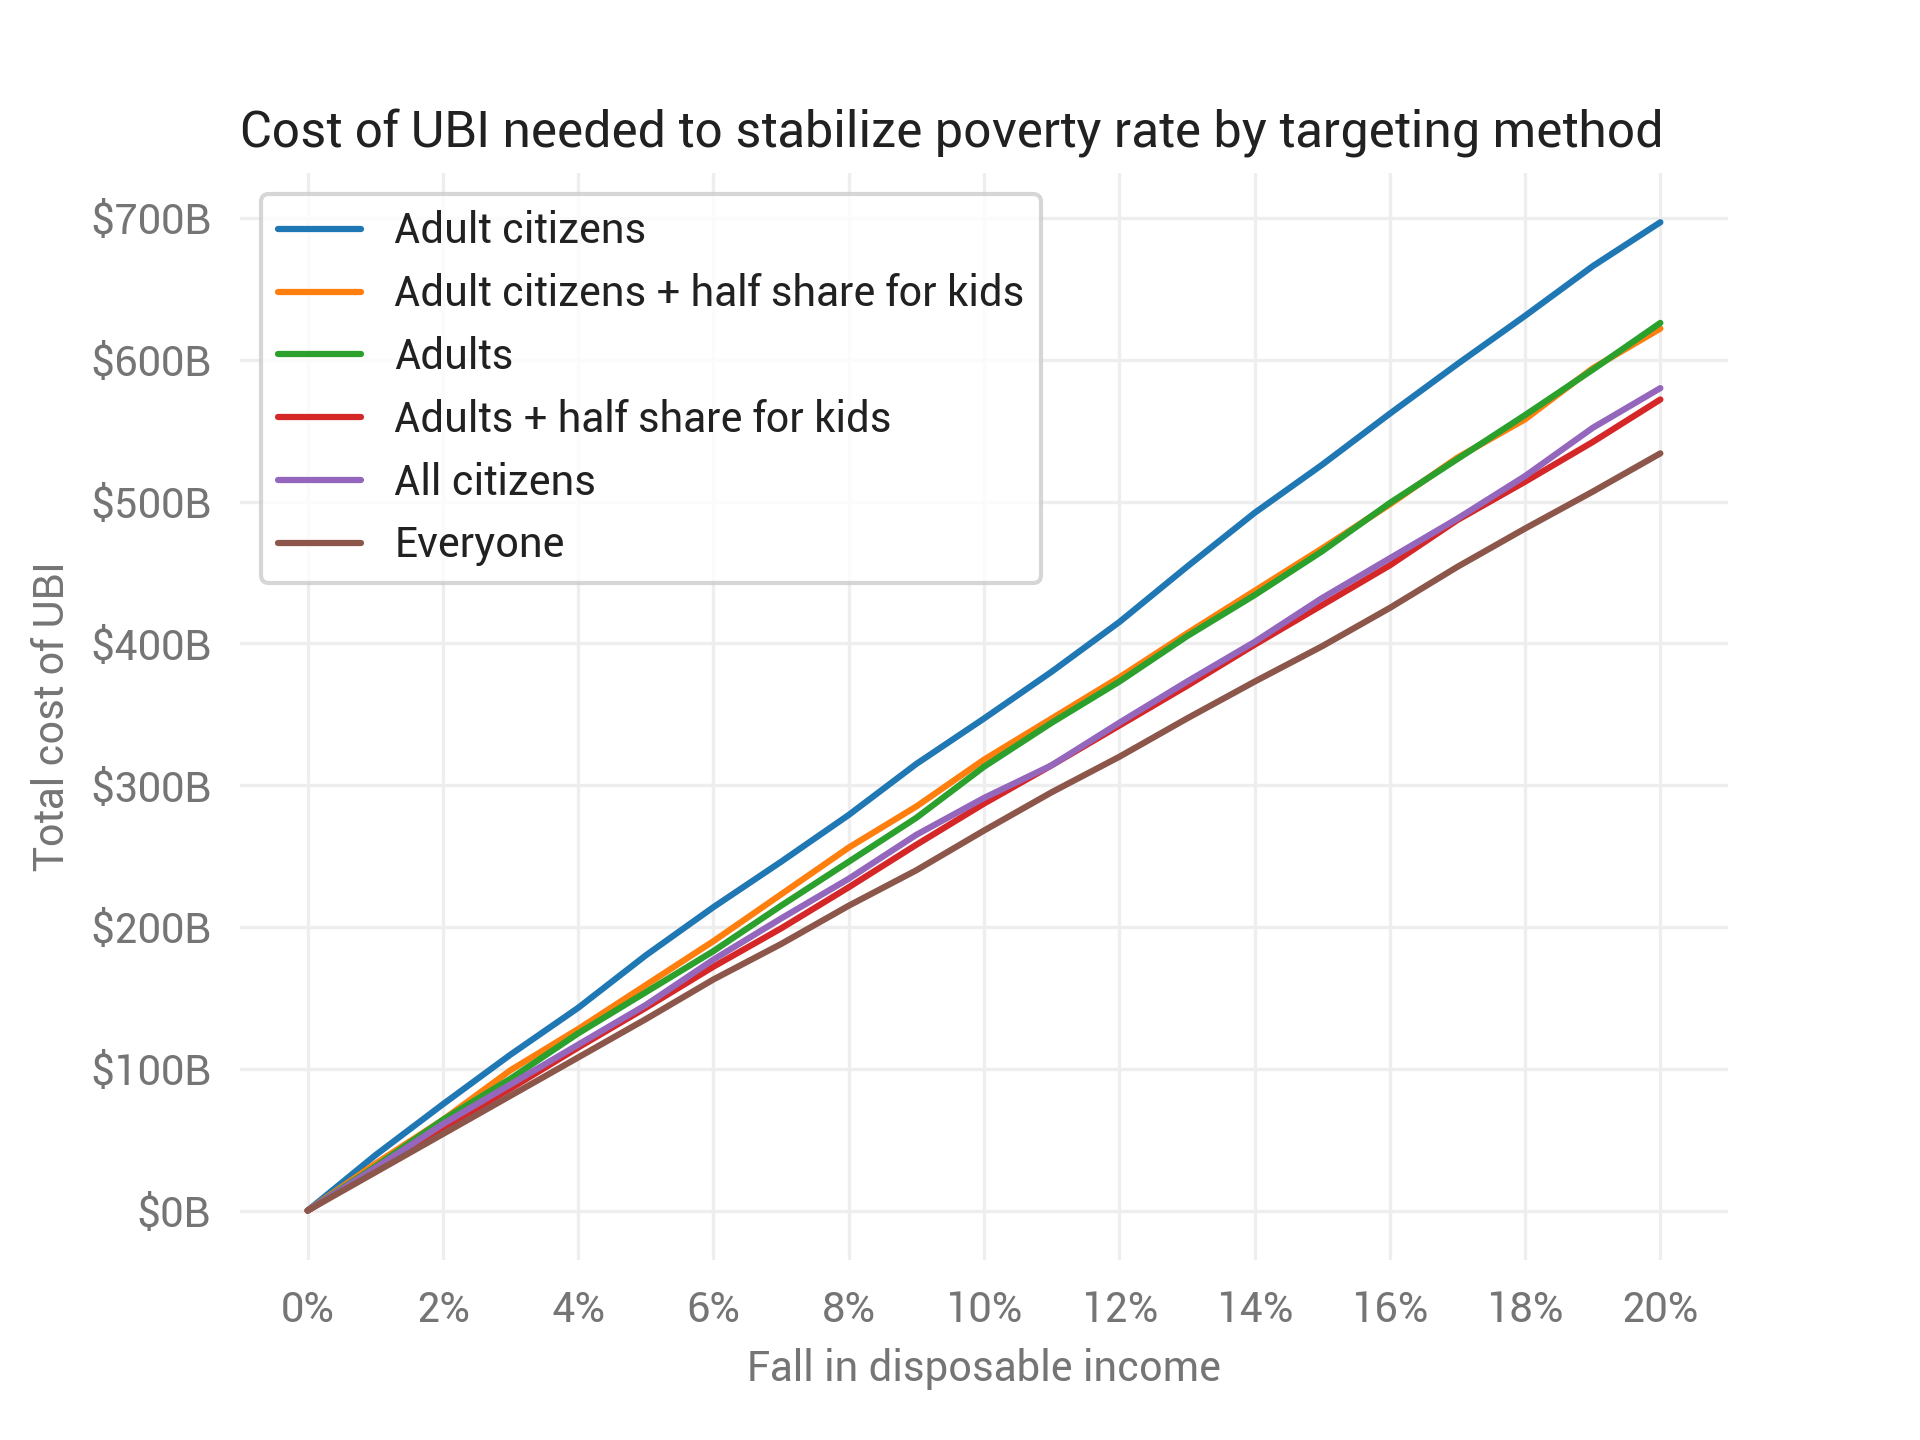
\includegraphics[width=15cm]{ubi_cost_pov_rate.png}
\captionof{figure}{}
\label{fig:ubi_cost_pov_rate}
\end{center}

\section{Conclusion} \label{sec:conclusion}

This paper quantifies the UBI amount necessary to stabilize the SPM poverty rate amid broad income drops. I find that modest payments can avert a rise in poverty; for example, if income falls by 10 percent, \$828 per person across all people, or \$1,515 if limited to adult citizens. The lower per-recipient cost of broad transfers outweighs the larger number of recipients, making them a cheaper path to poverty stabilization.

More generous UBIs than those needed to stabilize poverty may still be warranted, especially as part of a large stimulus package. Congress and the White House are expected to pass such a package in the coming days or weeks, likely including other policies like payroll tax cuts, paid sick leave, and assistance for airlines and small businesses. Compared to a budget-neutral UBI, these policies are likely to be regressive and exclusionary, though they could have other benefits like reducing unemployment, business closure, and infection.

Future research could substantially refine these findings by better modeling the real economic effects of the Covid-19 outbreak.

For example, we could start with a more realistic baseline poverty rate. From February 2018 to February 2020 (the latest data available), the prime-age employment ratio (ages 25 to 54) rose by 1.2 percentage points~\cite{fred_paepop} and real average weekly earnings rose by 2.4 percent~\cite{bls_earnings}. These data suggest that the SPM rate may have continued its fall from 2012 to 2018, and fallen further from 2018 to pre-pandemic 2020.

The UBI could also be inflation-adjusted to reflect the 3.9 percent rise in the Consumer Price Index from February 2018 to February 2020.\footnote{CPI-U rose from 248.991 in February 2018 to 258.678 in February 2020~\cite{bls_cpi_data}. The March 2020 CPI will be released on April 10~\cite{bls_cpi_releases}.} The \citeA{census_proj} additionally projects a population increase from 327.9 million in 2018 to 332.6 million in 2020. These factors combined suggest that the aggregate cost would be 5.4 percent higher in 2020 than the model this paper provides using 2018 data.

Once wage and employment data are released, the income reductions in this 2018 CPS data could be calibrated to those real-world changes. Translating wage and employment data to SPM resources requires some knowledge of how existing programs, such as unemployment insurance and food benefits including the Supplemental Nutrition Assistance Program, are administered. It could be further refined by considering heterogeneous income effects---for example, if service workers are hit particularly hard---but this would ultimately involve considerable rough estimation. The March 2020 Current Population Survey employment situation will be released on April 3~\cite{bls_releases}, reflecting employment for the week of March 8 to 14.\footnote{Respondents are asked about employment for the calendar week including the 12th day of each month~\cite{bls_cps_faq}.} A simple step in this direction would be excluding stable forms of income, such as Social Security payments, from the loss simulation.

Comparison to other interventions would also be useful. For example, halving 2020 payroll tax liabilities would have a roughly flat distributional impact as a share of income~\cite{taxbrain}, while a UBI would be highly progressive~\cite{ghenis_yang}.

Some cash proposals involve means-testing, which relies on untimely income information. The fastest way to means-test would be to use 2019 income tax returns, which reflect income from 2018 and are already available. This could improperly exclude people whose income fell from 2018 to mid-2020. Using tax returns for the calendar year 2019 would produce fewer exclusion errors, but payments would be delayed for people who haven't yet filed those returns---especially as the \citeA{irs} extended their payment deadline from April 15 to July 15. Whether using 2018 or 2019 returns, nonfilers would require special treatment that could cause further delays among those in greatest need. \citeA{ritz} instead propose sending universal checks immediately, and recovering amounts in 2020 tax filing next year, effectively structuring the payments as refundable tax credits or zero-interest loans, depending on income.

As incomes fall, a variety of policy options will help affected people in different circumstances. Paid sick leave will help workers who fall ill and whose employers don't currently offer it. Payroll tax cuts will increase take-home pay for salaried or wage workers. Bank assistance, loans, and grants will help business owners stay afloat and keep workers employed. Extending unemployment insurance and assistance programs will help those who suddenly lose income. But self-employed people, independent contractors, students who had to quickly relocate, and others facing new costs or employment hurdles are likely to fall through the cracks of even a comprehensive web of targeted programs.

UBI policies are well positioned to help all people with the urgency required of this crisis. Cash can be distributed immediately, especially if it's done broadly. Unlike in-kind benefits like food stamps, it can be used to pay any bills that arise. And as this paper shows, UBI is a cost-effective tool to prevent a rise in poverty. To maximize the anti-poverty impact, we should send checks broadly, generously, and quickly.

\appendix
\section{Poverty gap results} \label{sec:appendixa}

The 2018 SPM poverty gap is \$170 billion; that is, among the 12.7 percent of people in poverty, the aggregate difference between their resources and their poverty line equals \$170 billion. This equals \$524 per person in poverty, or \$4,116 per US resident.

If annual disposable incomes fell by 10 percent, the poverty gap would rise 14 percent.

\begin{center}
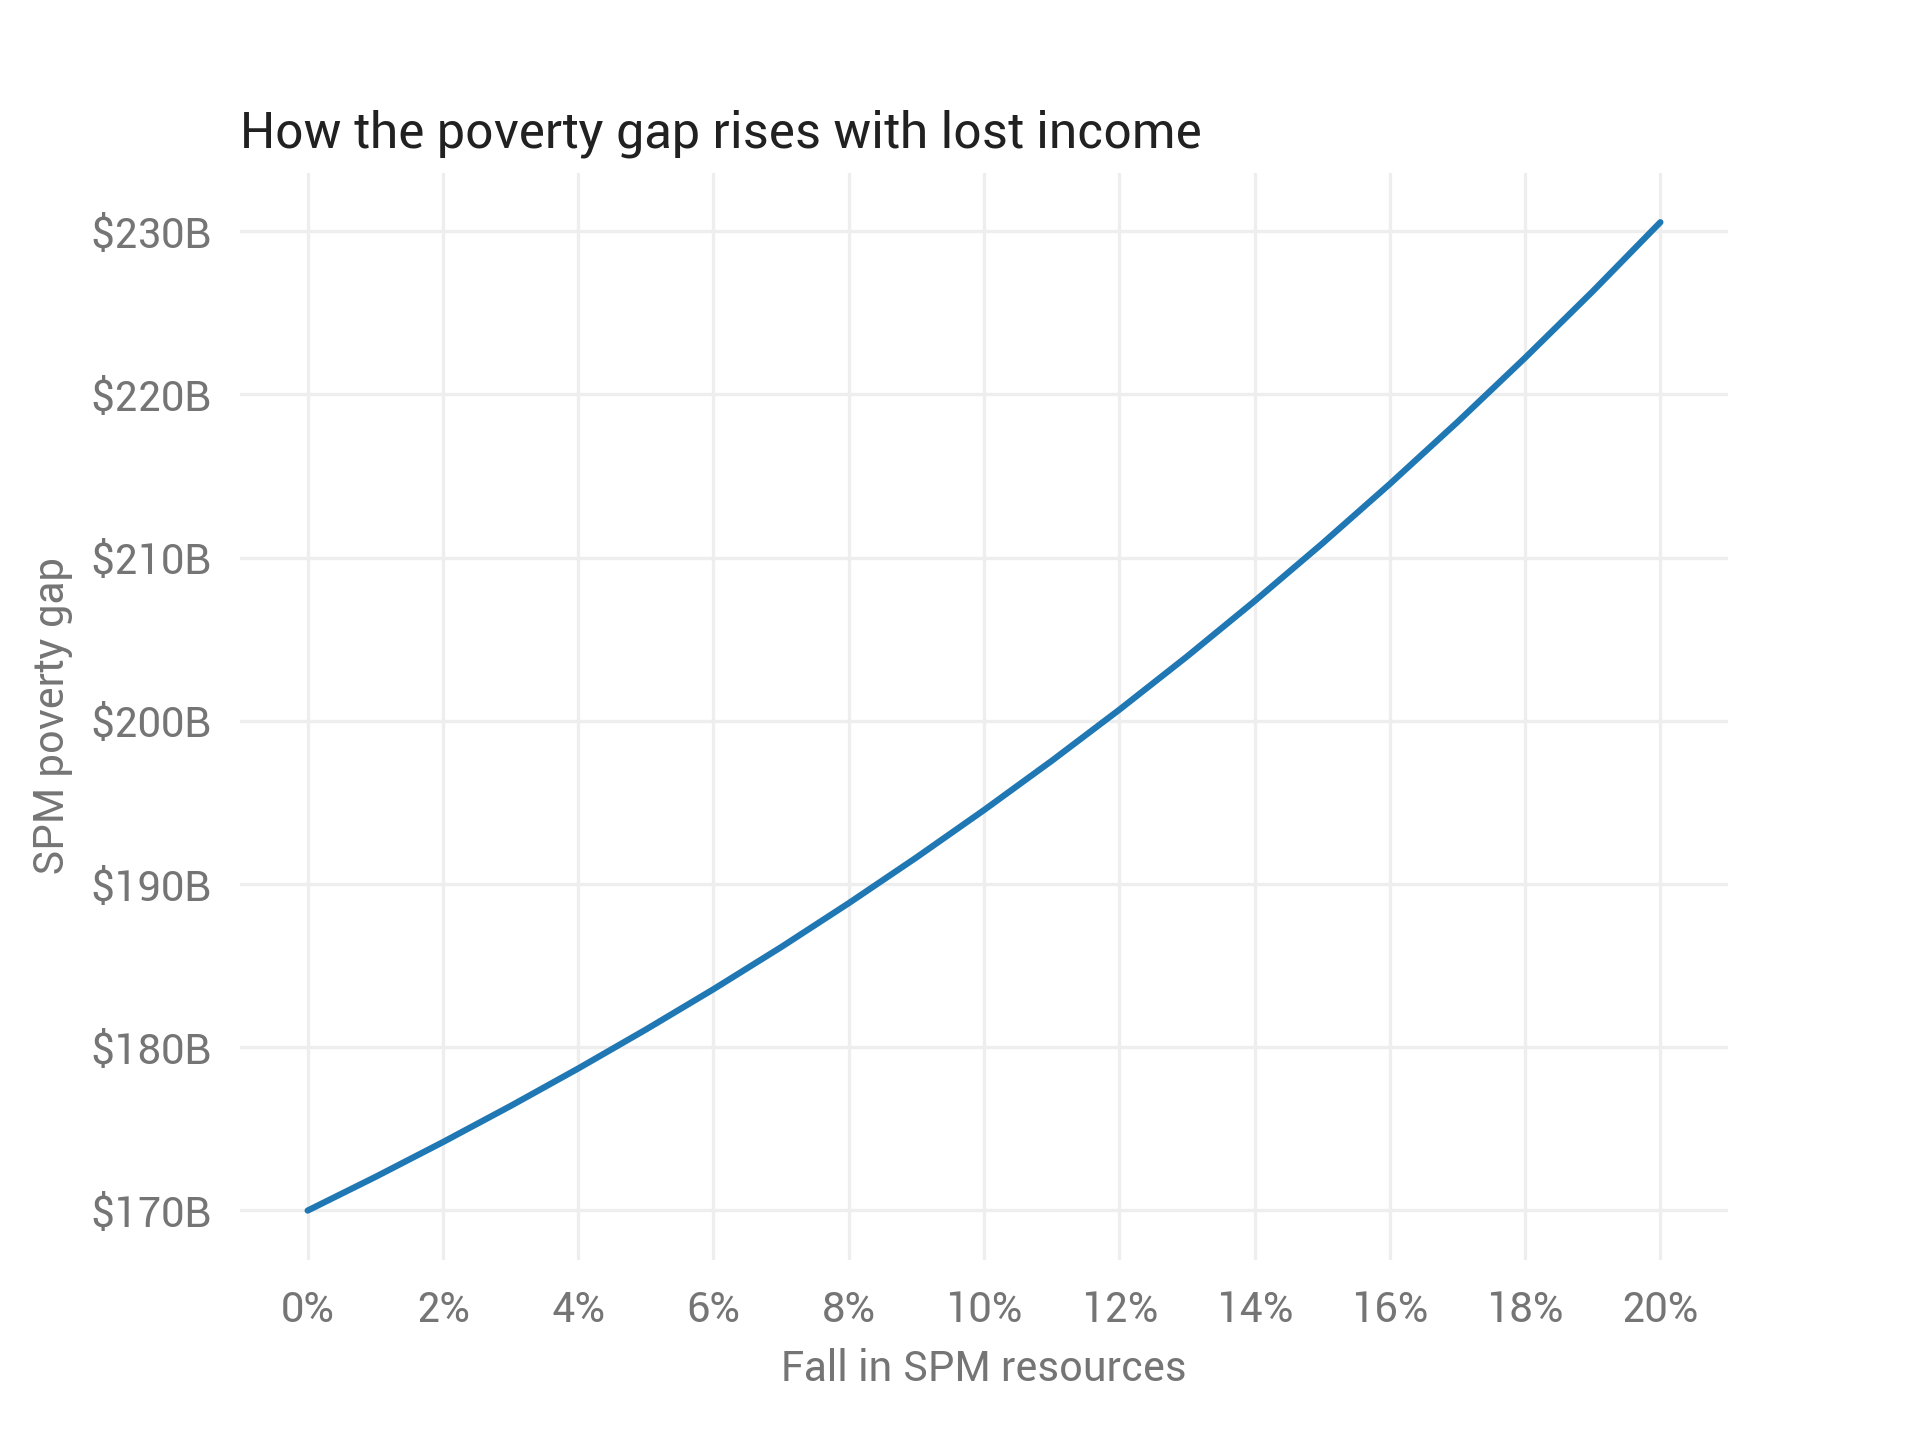
\includegraphics[width=15cm]{pov_gap_income.png}
\captionof{figure}{}
\label{fig:pov_gap_income}
\end{center}

Given 10 percent income losses, the UBI amount needed to stabilize the poverty gap is about a third lower than the UBI amount needed to stabilize the poverty rate.

\begin{center}
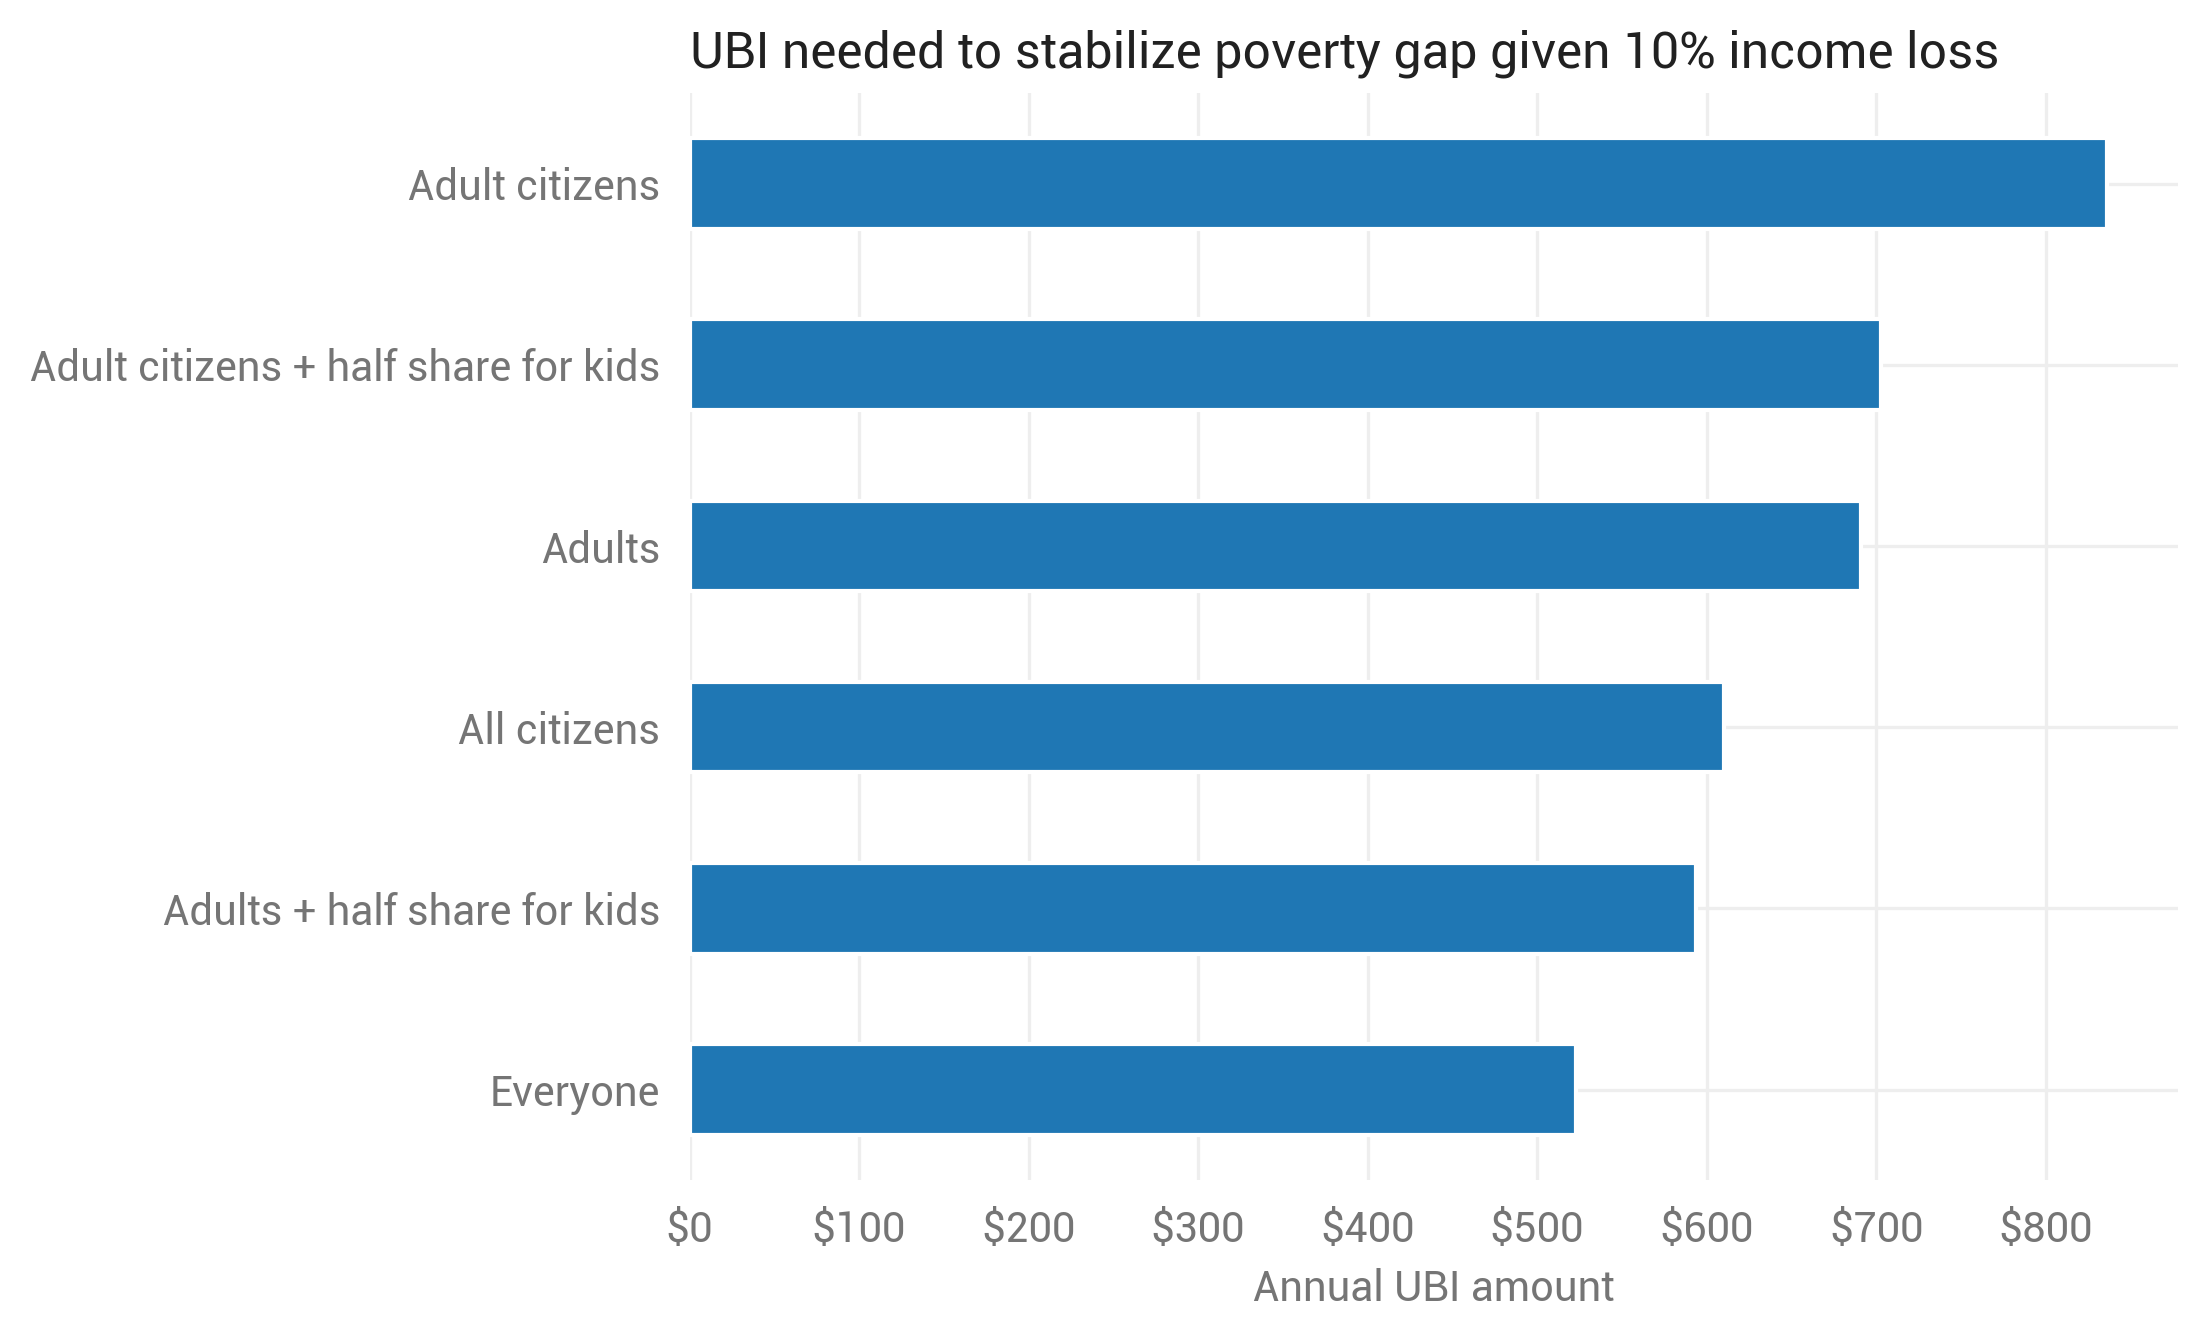
\includegraphics[width=15cm]{ubi_pov_gap_10pct.png}
\captionof{figure}{}
\label{fig:ubi_pov_gap_10pct}
\end{center}

This translates to a total cost of about a third lower, though the core finding from the poverty rate analysis---that including everyone is cheaper than restricting receipt---holds for the poverty gap as well.

\begin{center}
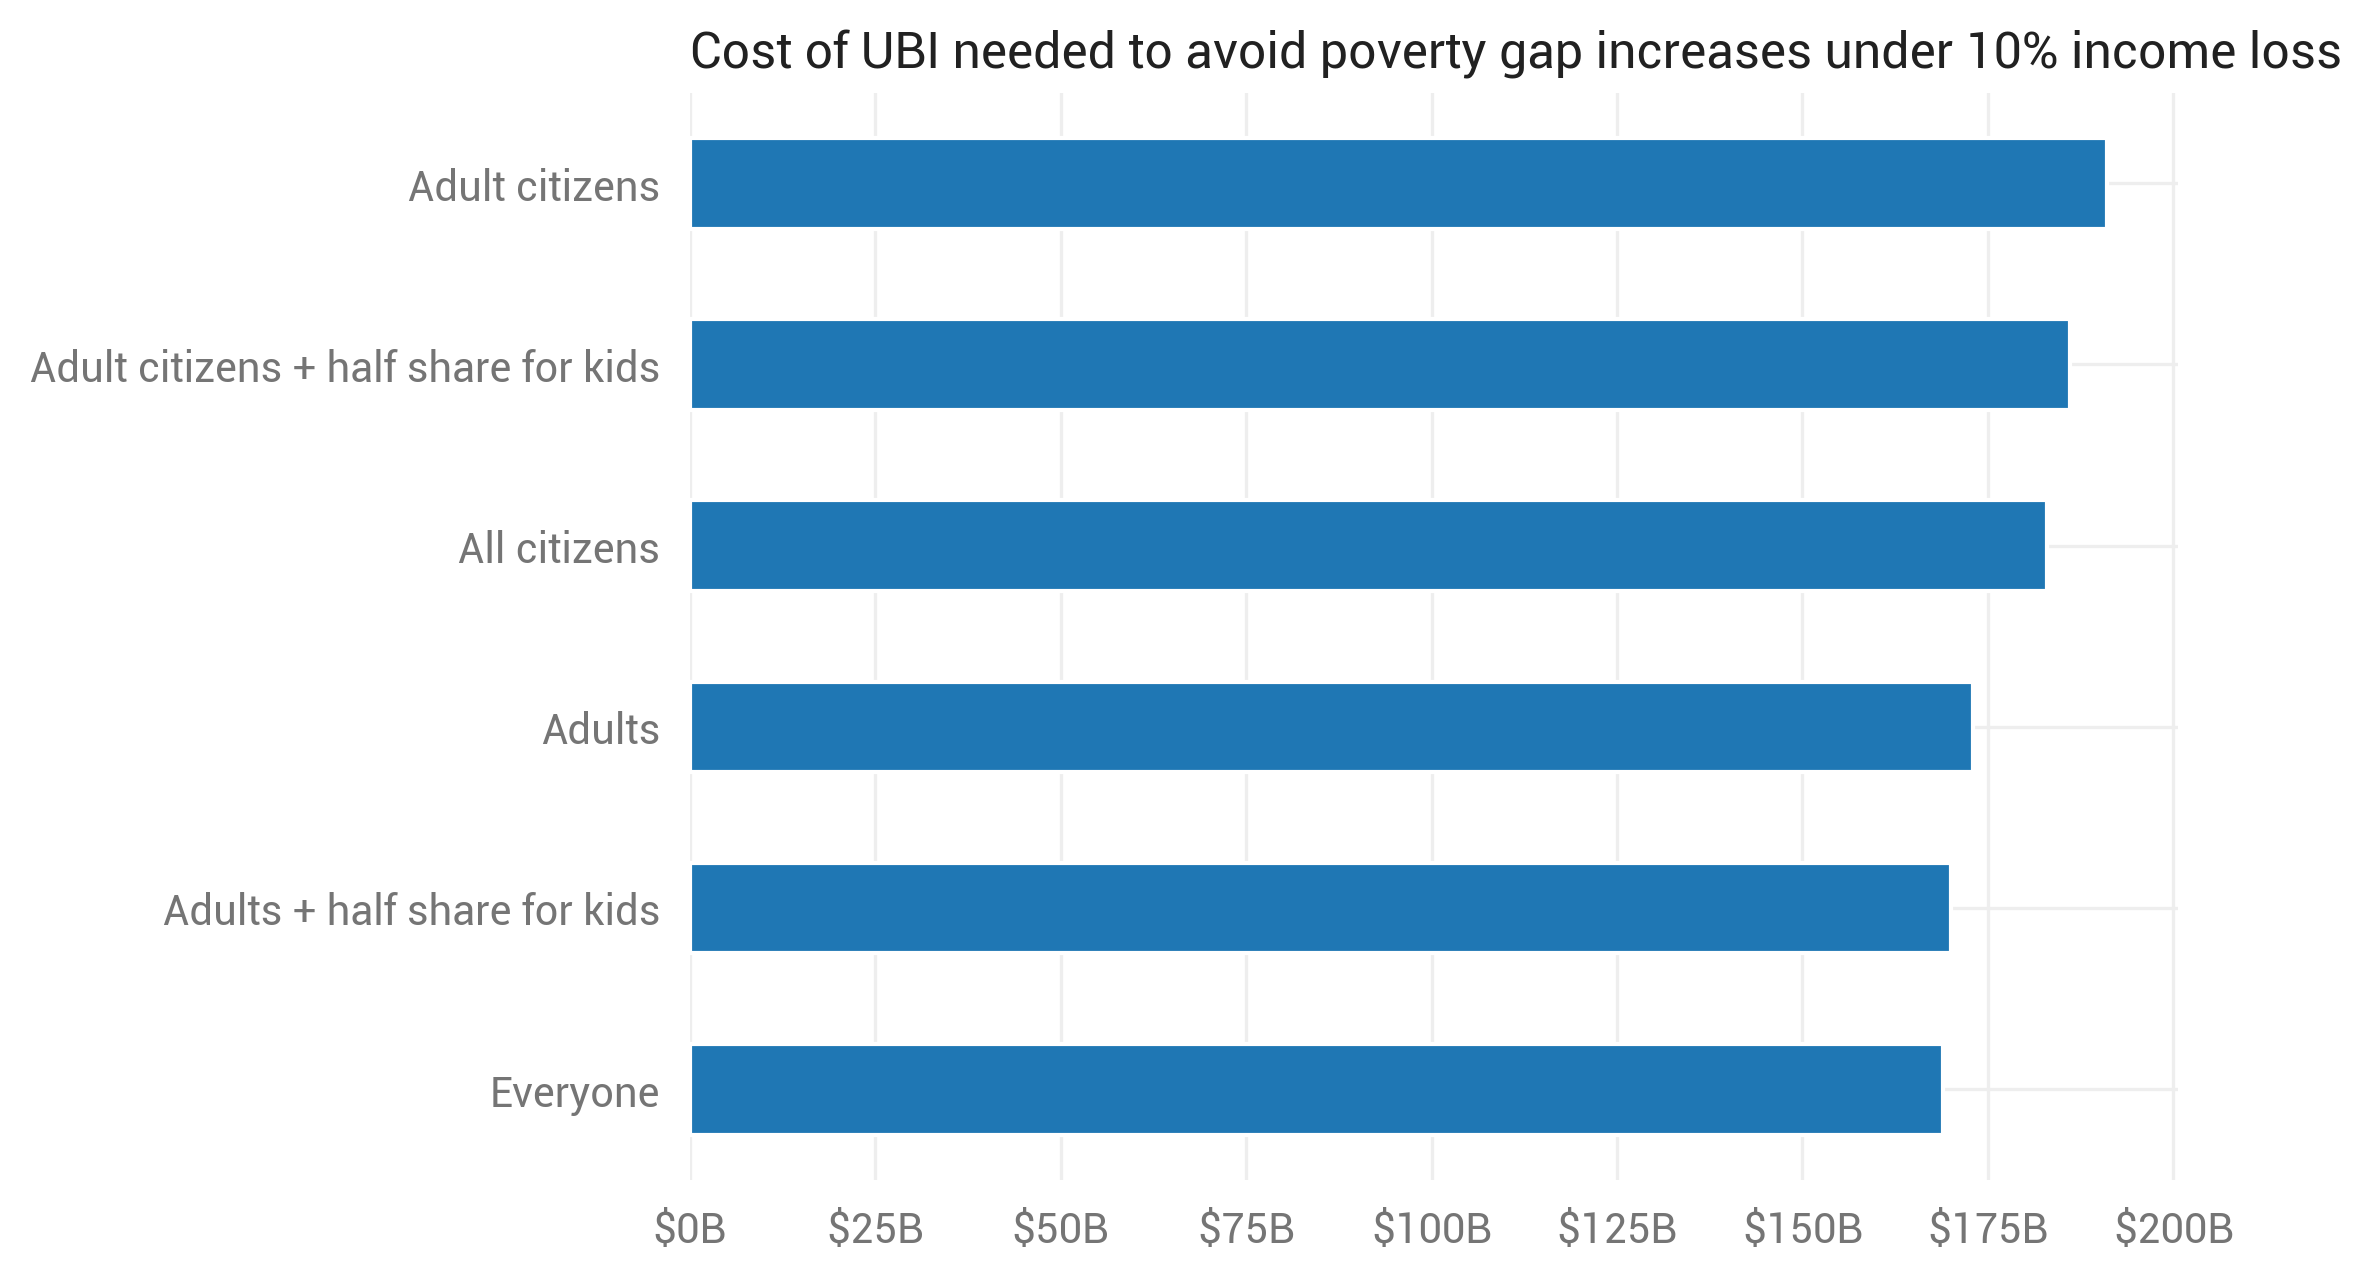
\includegraphics[width=15cm]{ubi_cost_pov_gap_10pct.png}
\captionof{figure}{}
\label{fig:ubi_cost_pov_gap_10pct}
\end{center}

The UBI amount is about a third lower than the poverty rate case across the range of potential income drops.

\begin{center}
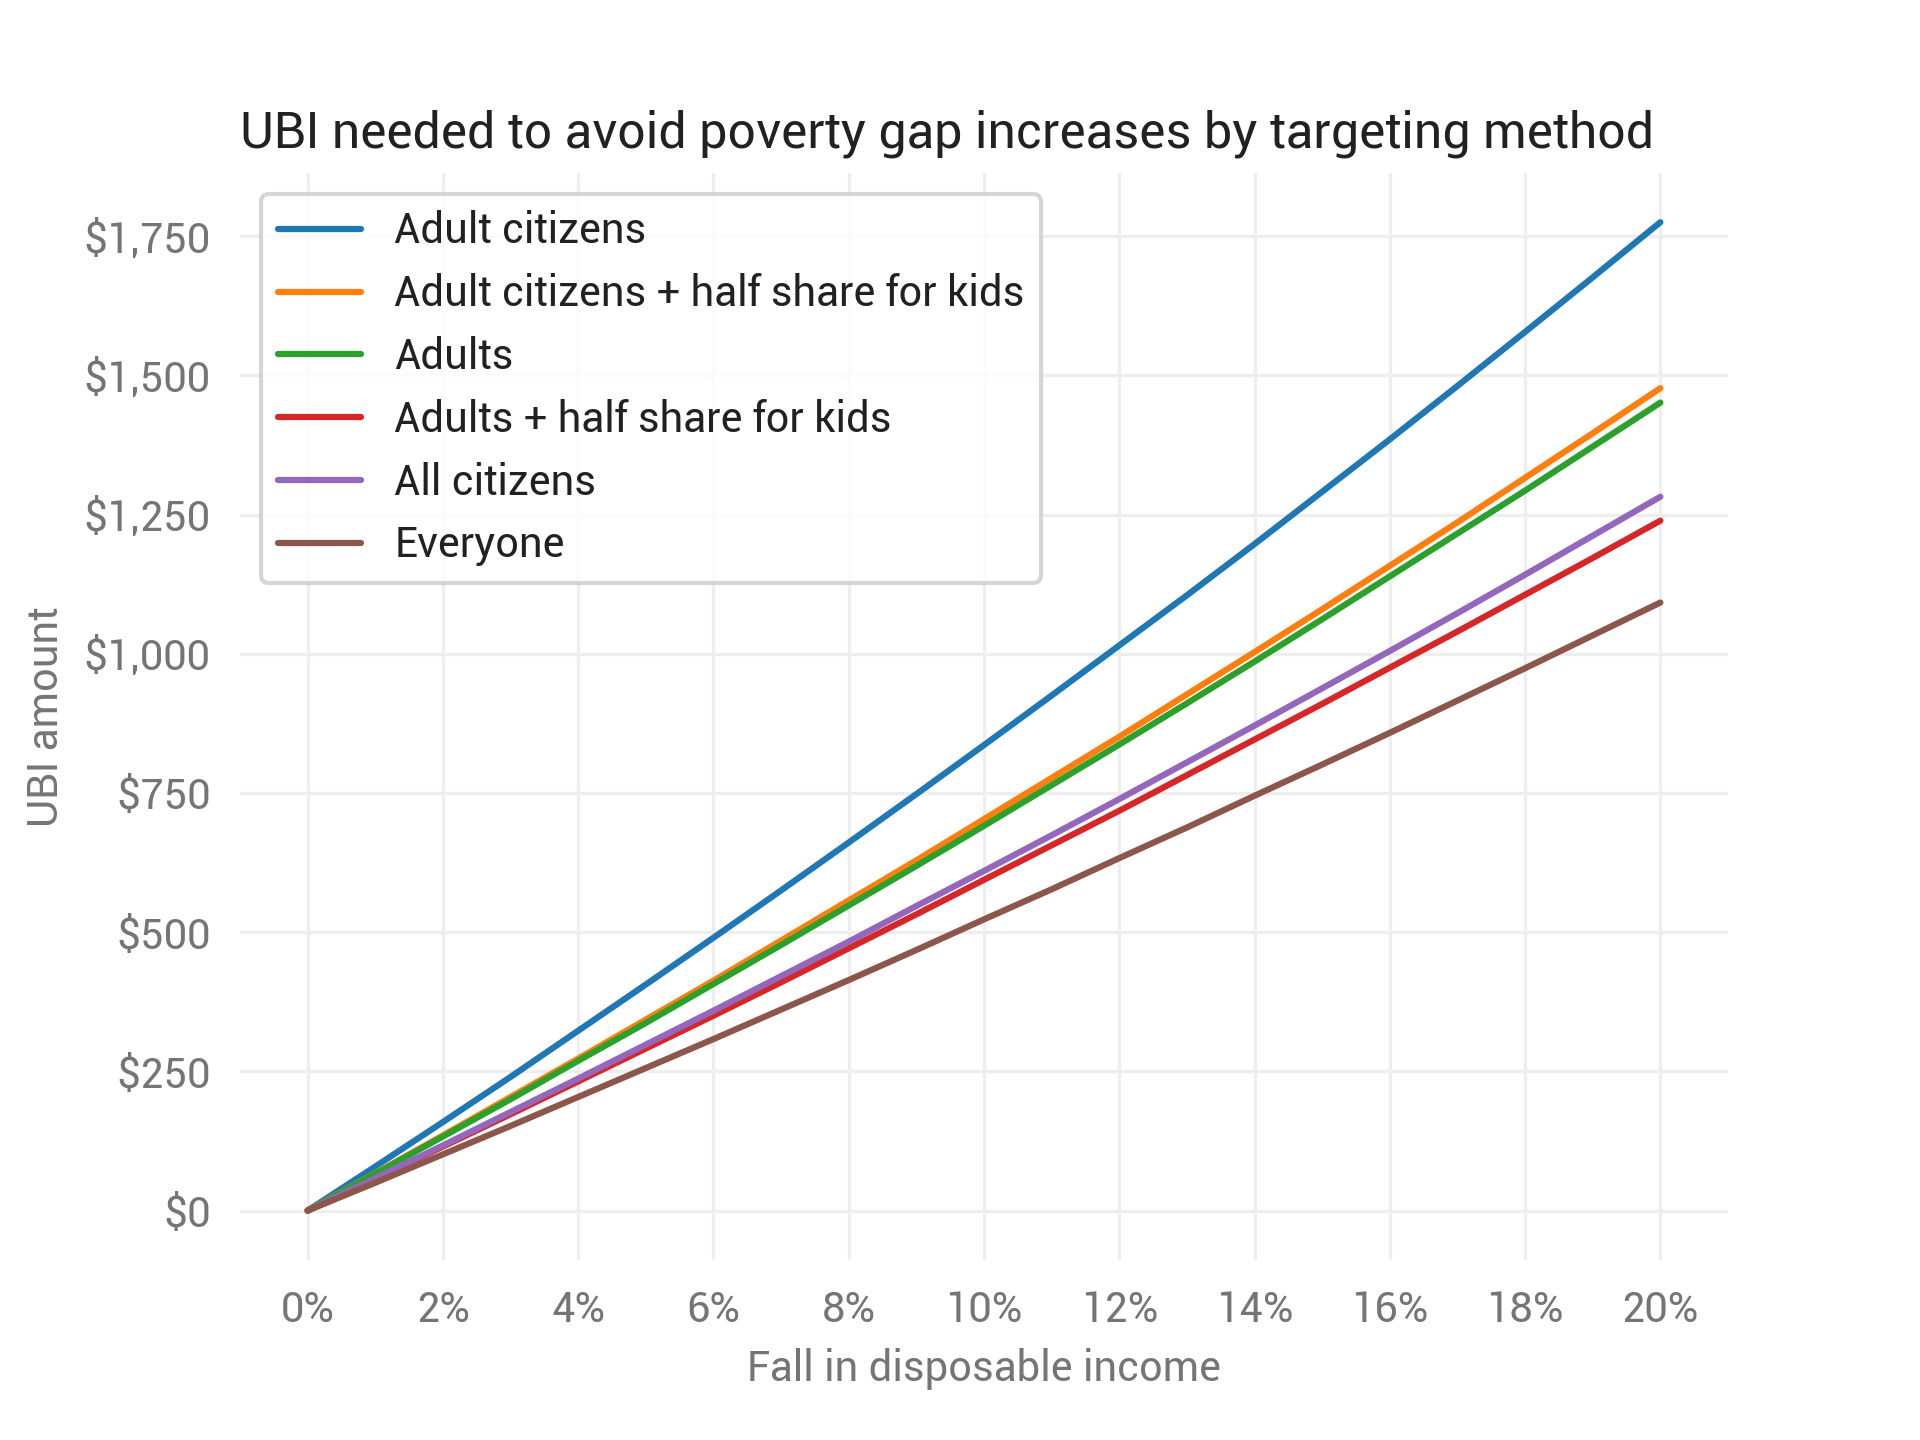
\includegraphics[width=15cm]{ubi_pov_gap.png}
\captionof{figure}{}
\label{fig:ubi_pov_gap}
\end{center}

Distributing the UBI to everyone is also more cost-effective regardless of the income drop, though the differences are smaller than in the poverty rate case.

\begin{center}
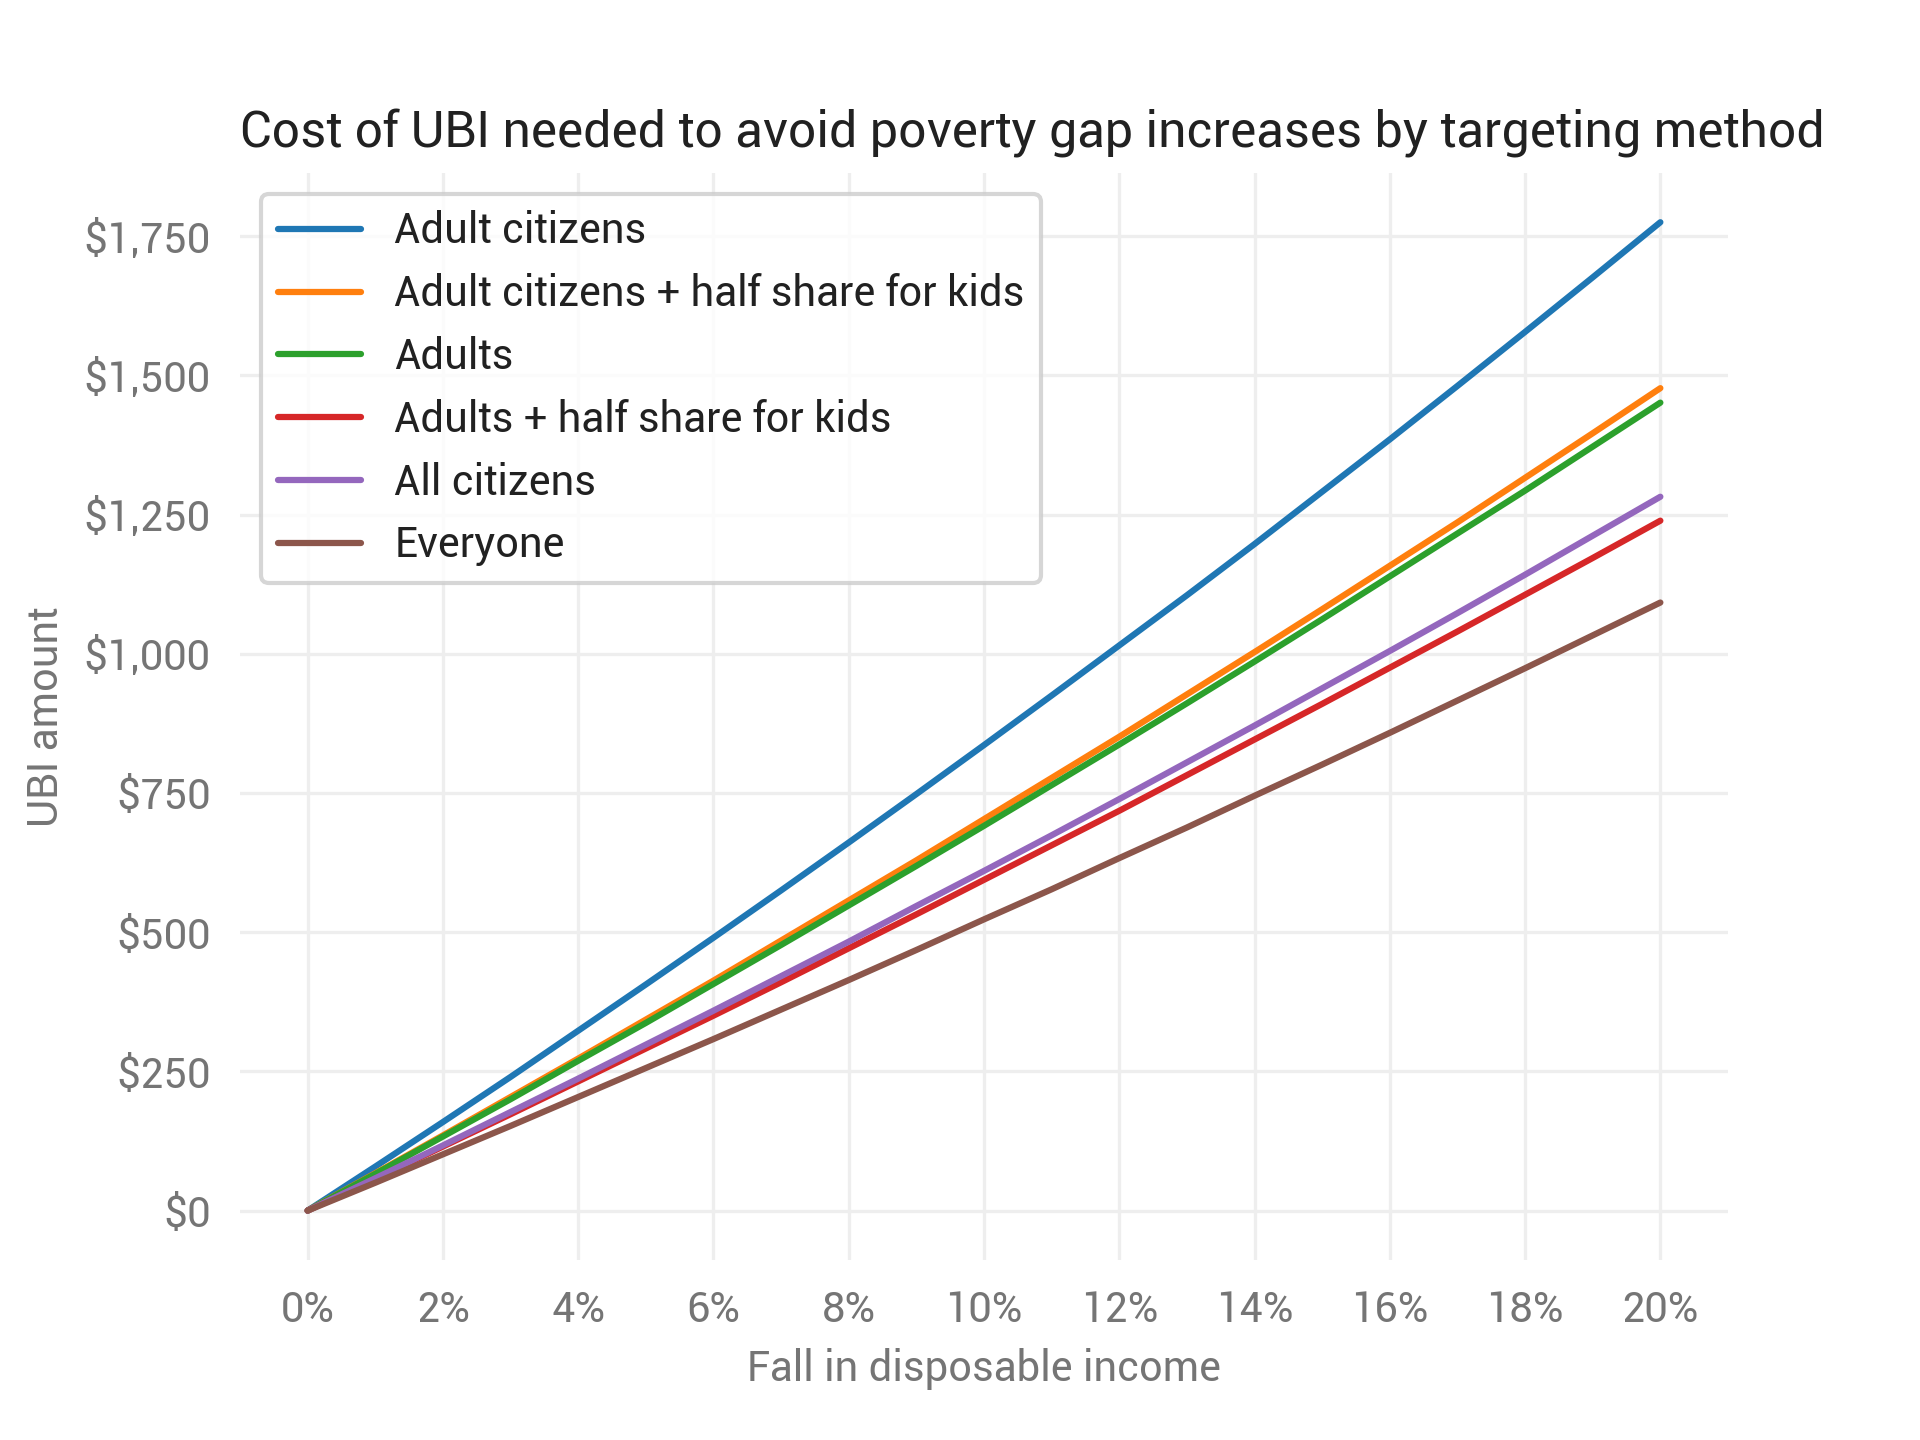
\includegraphics[width=15cm]{ubi_cost_pov_gap.png}
\captionof{figure}{}
\label{fig:ubi_cost_pov_gap}
\end{center}



\clearpage

%\singlespacing
%\setlength\bibsep{0pt}

\bibliographystyle{apacite}  % We choose the "plain" reference style.
\bibliography{refs}  % Entries are in the "refs.bib" file.

\end{document}
